%%%%%%%%%%%%%%%%%%%%%%%%%%%%%%%%%%%%%%%%%%%%%%%%%%%%%%%%%%%%%%%%%%%%%%%%%%%%%%%%%%%%%%%%%%
\begin{document}
\maketitle
%%%%%%%%%%%%%%%%%%%%%%%%%%%%%%%%%%%%%%%%%%%%%%%%%%%%%%%%%%%%%%%%%%%%%%%%%%%%%%%%%%%%%%%%%%

\begin{frame}
 \frametitle{Outline}
  \vspace{-1cm}
  1. Introduction\\[0.1cm]
  2. Mathematical Model\\[0.1cm]
  3. Validation\\[0.1cm]
  4. Results\\[0.1cm]
  5. Conclusion
\end{frame}


%%%%%%%%%%%%%%%%%%%%%%%%%%%%%%%%%%%%%%%%%%%%%%%%%%%%%%%%%%%%%%%%%%%%%%%%%%%%%%%%%%%%%%%%%

\begin{frame}
\frametitle{Introduction}
\vspace{-1.1cm}
\begin{columns}[c]
\column{.6\textwidth}
Motivation:
\begin{itemize}
  \justifying
  \item Ischaemic heart disease and stroke have remained the leading death causes globally in the last 15 years [1]
\end{itemize}
 
\vspace{0.5cm}
 
Aims:
\begin{itemize}
 \justifying
 \item To develop a Finite Element code for stream-vorticity formulation 
       with species transport equation using the Arbitrary Lagrangian-Eulerian (ALE) approach \\


 \vspace{0.2cm}
 \item To create new drug-eluting design patent 

\end{itemize}
\column{.4\textwidth}
\begin{center}
  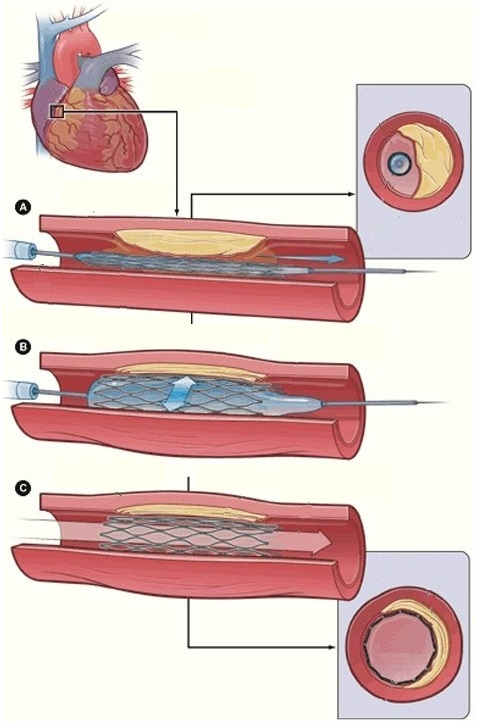
\includegraphics[scale=0.38]{images/stent_bare.jpg}
\end{center}
\end{columns}

\vspace{0.3cm}
\tiny [1] World Health Organization, 2018, "The top 10 causes of death".
\textit{www.who.int/news-room/fact-sheets/detail/the-top-10-causes-of-death}
[Online accessed 06-04-20 08:27pm]



\end{frame}


%%%%%%%%%%%%%%%%%%%%%%%%%%%%%%%%%%%%%%%%%%%%%%%%%%%%%%%%%%%%%%%%%%%%%%%%%%%%%%%%%%%%%%%%%%

\begin{frame}
  \vspace{-1cm}
  \textcolor{gray}{1. Introduction}\\[0.1cm]
  2. Mathematical Model\\[0.1cm]
  \textcolor{gray}{3. Validation}\\[0.1cm]
  \textcolor{gray}{4. Results}\\[0.1cm]
  \textcolor{gray}{5. Conclusion}
\end{frame}

%%%%%%%%%%%%%%%%%%%%%%%%%%%%%%%%%%%%%%%%%%%%%%%%%%%%%%%%%%%%%%%%%%%%%%%%%%%%%%%%%%%%%%%%%%


\begin{frame}
\frametitle{\LARGE Arbitrary Lagrangian-Eulerian (ALE)}
\vspace{-0.5cm}
\begin{columns}[c]
\column{.4\textwidth}
\justifying
In ALE description, the referential frame moves with an arbitrary velocity that does not necessary represents the Lagrangian or Eulerian description.

\bigskip
The convection velocity is calculated by the relative velocity between the material and the mesh velocity respectively [2]


\column{.5\textwidth}
\begin{center}
\begin{tikzpicture}[scale=0.8]

 % (a) Lagrangian
 % -------------------------------------------------------------------
 % bottom line
 \draw (0,5) -- (6,5);

 \node[square, fill=white, draw, inner sep=0pt, minimum size=8pt] at (0,5) {};
 \node[square, fill=white, draw, inner sep=0pt, minimum size=8pt] at (1,5) {};
 \node[square, fill=white, draw, inner sep=0pt, minimum size=8pt] at (2.7,5) {};
 \node[square, fill=white, draw, inner sep=0pt, minimum size=8pt] at (4,5) {};
 \node[square, fill=white, draw, inner sep=0pt, minimum size=8pt] at (5.1,5) {};
 \node[square, fill=white, draw, inner sep=0pt, minimum size=8pt] at (6,5) {};

 \node[circle, fill=black, inner sep=0pt, minimum size=4pt] at (0,5) {};
 \node[circle, fill=black, inner sep=0pt, minimum size=4pt] at (1,5) {};
 \node[circle, fill=black, inner sep=0pt, minimum size=4pt] at (2.7,5) {};
 \node[circle, fill=black, inner sep=0pt, minimum size=4pt] at (4,5) {};
 \node[circle, fill=black, inner sep=0pt, minimum size=4pt] at (5.1,5) {};
 \node[circle, fill=black, inner sep=0pt, minimum size=4pt] at (6.0,5) {};

 % top line
 \draw (0.5,6) -- (5.4,6);

 \node[square, fill=white, draw, inner sep=0pt, minimum size=8pt] at (0.5,6) {};
 \node[square, fill=white, draw, inner sep=0pt, minimum size=8pt] at (1.4,6) {};
 \node[square, fill=white, draw, inner sep=0pt, minimum size=8pt] at (2.3,6) {};
 \node[square, fill=white, draw, inner sep=0pt, minimum size=8pt] at (3.5,6) {};
 \node[square, fill=white, draw, inner sep=0pt, minimum size=8pt] at (4.6,6) {};
 \node[square, fill=white, draw, inner sep=0pt, minimum size=8pt] at (5.4,6) {};

 \node[circle, fill=black, inner sep=0pt, minimum size=4pt] at (0.5,6) {};
 \node[circle, fill=black, inner sep=0pt, minimum size=4pt] at (1.4,6) {};
 \node[circle, fill=black, inner sep=0pt, minimum size=4pt] at (2.3,6){};
 \node[circle, fill=black, inner sep=0pt, minimum size=4pt] at (3.5,6) {};
 \node[circle, fill=black, inner sep=0pt, minimum size=4pt] at (4.6,6) {};
 \node[circle, fill=black, inner sep=0pt, minimum size=4pt] at (5.4,6) {};

 % mesh motion
 \draw [dashed] (0,  5) -- (0.5,6)  ;
 \draw [dashed] (1,  5) -- (1.4,6)  ;
 \draw [dashed] (2.7,5) -- (2.3,6);
 \draw [dashed] (4,  5) -- (3.5,6)  ;
 \draw [dashed] (5.1,5) -- (4.6,6);
 \draw [dashed] (6,  5) -- (5.4,6)  ;

 % particle motion
 \draw [dotted] (0,  5.15) -- (0.5,5.85);
 \draw [dotted] (1,  5.15) -- (1.4,5.85);
 \draw [dotted] (2.7,5.15) -- (2.3,5.85);
 \draw [dotted] (4,  5.15) -- (3.5,5.85);
 \draw [dotted] (5.1,5.15) -- (4.6,5.85);
 \draw [dotted] (6,  5.15) -- (5.4,5.85):



 % Eulerian legend 
 \draw [latexnew-latex] (-0.3,5) -- (-0.3,6);
 \node at (-0.5,5.5) {t};
 \node at (3,6.5) {\scriptsize Lagrangian description};
 % -------------------------------------------------------------------
 


 % (b) Eulerian
 % -------------------------------------------------------------------
 % bottom line
 \draw (0,2.5) -- (6,2.5);

 \node[square, fill=white, draw, inner sep=0pt, minimum size=8pt] at (0,2.5) {};
 \node[square, fill=white, draw, inner sep=0pt, minimum size=8pt] at (1,2.5) {};
 \node[square, fill=white, draw, inner sep=0pt, minimum size=8pt] at (2.7,2.5) {};
 \node[square, fill=white, draw, inner sep=0pt, minimum size=8pt] at (4,2.5) {};
 \node[square, fill=white, draw, inner sep=0pt, minimum size=8pt] at (5.1,2.5) {};
 \node[square, fill=white, draw, inner sep=0pt, minimum size=8pt] at (6,2.5) {};

 \node[circle, fill=black, inner sep=0pt, minimum size=4pt] at (0,  2.5) {};
 \node[circle, fill=black, inner sep=0pt, minimum size=4pt] at (1,  2.5) {};
 \node[circle, fill=black, inner sep=0pt, minimum size=4pt] at (2.7,2.5) {};
 \node[circle, fill=black, inner sep=0pt, minimum size=4pt] at (4,  2.5) {};
 \node[circle, fill=black, inner sep=0pt, minimum size=4pt] at (5.1,2.5) {};
 \node[circle, fill=black, inner sep=0pt, minimum size=4pt] at (6.0,2.5) {};

 % top line
 \draw (0,3.5) -- (6,3.5);

 \node[square, fill=white, draw, inner sep=0pt, minimum size=8pt] at (0.5,3.5) {};
 \node[square, fill=white, draw, inner sep=0pt, minimum size=8pt] at (1.4,3.5) {};
 \node[square, fill=white, draw, inner sep=0pt, minimum size=8pt] at (2.3,3.5) {};
 \node[square, fill=white, draw, inner sep=0pt, minimum size=8pt] at (3.5,3.5) {};
 \node[square, fill=white, draw, inner sep=0pt, minimum size=8pt] at (4.6,3.5) {};
 \node[square, fill=white, draw, inner sep=0pt, minimum size=8pt] at (5.4,3.5) {};

 \node[circle, fill=black, inner sep=0pt, minimum size=4pt] at (0,  3.5) {};
 \node[circle, fill=black, inner sep=0pt, minimum size=4pt] at (1,  3.5) {};
 \node[circle, fill=black, inner sep=0pt, minimum size=4pt] at (2.7,3.5){};
 \node[circle, fill=black, inner sep=0pt, minimum size=4pt] at (4,  3.5) {};
 \node[circle, fill=black, inner sep=0pt, minimum size=4pt] at (5.1,3.5) {};
 \node[circle, fill=black, inner sep=0pt, minimum size=4pt] at (6.0,3.5) {};

 % mesh motion
 \draw [dashed] (0,  2.5) -- (0,  3.5)  ;
 \draw [dashed] (1,  2.5) -- (1,  3.5)  ;
 \draw [dashed] (2.7,2.5) -- (2.7,3.5)  ;
 \draw [dashed] (4,  2.5) -- (4,  3.5)  ;
 \draw [dashed] (5.1,2.5) -- (5.1,3.5)  ;
 \draw [dashed] (6,  2.5) -- (6,  3.5)  ;

 % particle motion
 \draw [dotted] (0,  2.65) -- (0.5,3.35);
 \draw [dotted] (1,  2.65) -- (1.4,3.35);
 \draw [dotted] (2.7,2.65) -- (2.3,3.35);
 \draw [dotted] (4,  2.65) -- (3.5,3.35);
 \draw [dotted] (5.1,2.65) -- (4.6,3.35);
 \draw [dotted] (6,  2.65) -- (5.4,3.35):



 % Eulerian legend 
 \draw [latexnew-latex] (-0.3,2.5) -- (-0.3,3.5);
 \node at (-0.5,3) {t};
 \node at (3,4.0) {\scriptsize Eulerian description};
 % -------------------------------------------------------------------
 


 % (c) ALE
 % -------------------------------------------------------------------
 % bottom line
 \draw (0,0) -- (6,0);

 \node[square, fill=white, draw, inner sep=0pt, minimum size=8pt] at (0,0) {};
 \node[square, fill=white, draw, inner sep=0pt, minimum size=8pt] at (1,0) {};
 \node[square, fill=white, draw, inner sep=0pt, minimum size=8pt] at (2.7,0) {};
 \node[square, fill=white, draw, inner sep=0pt, minimum size=8pt] at (4,0) {};
 \node[square, fill=white, draw, inner sep=0pt, minimum size=8pt] at (5.1,0) {};
 \node[square, fill=white, draw, inner sep=0pt, minimum size=8pt] at (6,0) {};

 \node[circle, fill=black, inner sep=0pt, minimum size=4pt] at (0,0) {};
 \node[circle, fill=black, inner sep=0pt, minimum size=4pt] at (1,0) {};
 \node[circle, fill=black, inner sep=0pt, minimum size=4pt] at (2.7,0) {};
 \node[circle, fill=black, inner sep=0pt, minimum size=4pt] at (4,0) {};
 \node[circle, fill=black, inner sep=0pt, minimum size=4pt] at (5.1,0) {};
 \node[circle, fill=black, inner sep=0pt, minimum size=4pt] at (6.0,0) {};

 % top line
 \draw (0.2,1) -- (5.8,1);

 \node[square, fill=white, draw, inner sep=0pt, minimum size=8pt] at (0.5,1) {};
 \node[square, fill=white, draw, inner sep=0pt, minimum size=8pt] at (1.4,1) {};
 \node[square, fill=white, draw, inner sep=0pt, minimum size=8pt] at (2.3,1) {};
 \node[square, fill=white, draw, inner sep=0pt, minimum size=8pt] at (3.5,1) {};
 \node[square, fill=white, draw, inner sep=0pt, minimum size=8pt] at (4.6,1) {};
 \node[square, fill=white, draw, inner sep=0pt, minimum size=8pt] at (5.4,1) {};

 \node[circle, fill=black, inner sep=0pt, minimum size=4pt] at (0.2,1) {};
 \node[circle, fill=black, inner sep=0pt, minimum size=4pt] at (1.1,1) {};
 \node[circle, fill=black, inner sep=0pt, minimum size=4pt] at (2.8,1) {};
 \node[circle, fill=black, inner sep=0pt, minimum size=4pt] at (3.8,1) {};
 \node[circle, fill=black, inner sep=0pt, minimum size=4pt] at (4.9,1) {};
 \node[circle, fill=black, inner sep=0pt, minimum size=4pt] at (5.8,1) {};

 % mesh motion
 \draw [dashed] (0,0.0) -- (0.2,1);
 \draw [dashed] (1,0.0) -- (1.1,1);
 \draw [dashed] (2.7,0.0) -- (2.8,1);
 \draw [dashed] (4,0.0) -- (3.8,1);
 \draw [dashed] (5.1,0.0) -- (4.9,1);
 \draw [dashed] (6,0.0) -- (5.8,1);

 % particle motion
 \draw [dotted] (0,0.15) -- (0.5,0.85);
 \draw [dotted] (1,0.15) -- (1.4,0.85);
 \draw [dotted] (2.7,0.15) -- (2.3,0.85);
 \draw [dotted] (4,0.15) -- (3.5,0.85);
 \draw [dotted] (5.1,0.15) -- (4.6,0.85);
 \draw [dotted] (6,0.15) -- (5.4,0.85):



 % ALE legend 
 \draw [latexnew-latex] (-0.3,0) -- (-0.3,1);
 \node at (-0.5,0.5) {t};
 \node at (3,1.5) {\scriptsize ALE description};
 

 % picture legend
 \node[square, draw, inner sep=0pt, minimum size=8pt] at (0.5,-0.7);
 \node[circle, fill=black, inner sep=0pt, minimum size=4pt] at (0.5,-1.2);
 \draw [dotted] (3.5,-0.7) -- (4.08,-0.7);
 \draw [dashed] (3.5,-1.2) -- (4.1,-1.2);

 \node at (1.7,-0.7) {\tiny material point};
 \node at (1.2,-1.2) {\tiny node};
 \node at (5.2,-0.7) {\tiny particle motion};
 \node at (5.1,-1.2) {\tiny mesh motion};
 % -------------------------------------------------------------------


\end{tikzpicture}
\end{center}
\end{columns}

\vspace{0.3cm}
\tiny [2]
Donea, J., Huerta, A., Ponthot, J.‐P. and Rodríguez‐Ferran, A. (2004). Arbitrary Lagrangian–Eulerian Methods. In Encyclopedia of Computational Mechanics \textit{doi:10.1002/0470091355.ecm009}
\end{frame}



%%%%%%%%%%%%%%%%%%%%%%%%%%%%%%%%%%%%%%%%%%%%%%%%%%%%%%%%%%%%%%%%%%%%%%%%%%%%%%%%%%%%%%%%%%

\begin{frame} 
 \frametitle{\LARGE Governing Equations}
\vspace{-1.2cm}
\begin{columns}[c]
\column{.6\textwidth}
Assumptions:\\[0.1cm]
\hspace{0.5cm}  1. Continuum hypothesis\\[0.1cm]
\hspace{0.5cm}  2. Homogeneous and Isotropic\\[0.1cm]
\hspace{0.5cm}  3. Incompressible\\[0.1cm]
\hspace{0.5cm}  4. Newtonian\\[0.1cm]
\hspace{0.5cm}  5. Constant Mass Difusivity\\[0.1cm]
\hspace{0.5cm}  6. Single-phase Flow\\[0.1cm]
\hspace{0.5cm}  7. Two-dimensional flow

\vspace{-1cm}
\column{.4\textwidth}
\begin{center}
\begin{equation*}
 \frac{D \omega}{Dt} = \frac{1}{Re} \nabla^{2} \omega
\end{equation*}
\medskip
\begin{equation*}
 \nabla^{2} \psi = - \omega
\end{equation*}
\medskip
\begin{equation*}
 \frac{Dc}{Dt} = \frac{1}{ReSc} \nabla^{2} c 
\end{equation*}
\end{center}
\end{columns}

\vspace{1.2cm}
\justifying
where, $D(\cdot)/Dt$ is substantive derivative and
the material velocity field is calculated by: 
$v_{x} = \partial \psi / \partial y$ and 
$v_{y} = - \partial \psi / \partial x$

\end{frame}



%%%%%%%%%%%%%%%%%%%%%%%%%%%%%%%%%%%%%%%%%%%%%%%%%%%%%%%%%%%%%%%%%%%%%%%%%%%%%%%%%%%%%%%%%%
\iffalse
\begin{frame}
 \frametitle{\LARGE Semi-Lagragian Method}

\vspace{-0.8cm}
\begin{columns}[c]
\column{.5\textwidth}
\justifying

\vspace{-1.4cm}
The figure (a) shows 1D space scheme of the semi-Lagrangian method.
The departure node is found by integration the mesh backward in time using $x_{i-1}$ and $x_{i}$

\vspace{2cm}
The figure (b) shows three possible trajectories of departure node
while developing the searching procedure


\column{.5\textwidth}
\begin{center}
\begin{tikzpicture}[scale=2.5]
 
 % grid
 \draw (2.5,2.5) -- (4.0,2.5);
 \draw (2.5,2.8) -- (4.0,2.8);
 \draw (2.5,3.0) -- (4.0,3.0);

 % material points
 \draw[dashed] (2.8,2.5) -- (3.12,2.8);
 \node[square, fill=white, draw, inner sep=0pt, minimum size=8pt] at (2.8,2.5) {};
 \node[square, fill=white, draw, inner sep=0pt, minimum size=8pt] at (3.12,2.8) {};
 

 % nodes
 \node[circle, fill=black, inner sep=0pt, minimum size=4pt] at (2.60,2.5) {};
 \node[circle, fill=black, inner sep=0pt, minimum size=4pt] at (3.12,2.5) {};
 \node[circle, fill=black, inner sep=0pt, minimum size=4pt] at (3.64,2.5) {};
 \node[circle, fill=black, inner sep=0pt, minimum size=4pt] at (3.90,2.5) {};

 \node[circle, fill=black, inner sep=0pt, minimum size=4pt] at (2.60,2.8) {};
 \node[circle, fill=black, inner sep=0pt, minimum size=4pt] at (3.12,2.8) {};
 \node[circle, fill=black, inner sep=0pt, minimum size=4pt] at (3.64,2.8) {};
 \node[circle, fill=black, inner sep=0pt, minimum size=4pt] at (3.90,2.8) {};

 \node[circle, fill=black, inner sep=0pt, minimum size=4pt] at (2.60,3.0) {};
 \node[circle, fill=black, inner sep=0pt, minimum size=4pt] at (3.12,3.0) {};
 \node[circle, fill=black, inner sep=0pt, minimum size=4pt] at (3.64,3.0) {};
 \node[circle, fill=black, inner sep=0pt, minimum size=4pt] at (3.90,3.0) {};


 % legend
 \node[draw=none, scale=0.8] at (2.80,2.62) {\small $\mathbf{x}_{d}$};
 \node[draw=none, scale=0.8] at (3.22,2.68) {\small $\mathbf{x}_{i}$};

 \node[draw=none, scale=0.8] at (4.10,2.50) {\small $t^{n}$};
 \node[draw=none, scale=0.8] at (4.15,2.80) {\small $t^{n+1}$};
 \node[draw=none, scale=0.8] at (4.15,3.00) {\small $t^{n+2}$};

 \node[draw=none, scale=0.8] at (2.60,2.35) {\small $\mathbf{x}_{i-1}$};
 \node[draw=none, scale=0.8] at (3.12,2.35) {\small $\mathbf{x}_{i}$};
 \node[draw=none, scale=0.8] at (3.64,2.35) {\small $\mathbf{x}_{i+1}$};
 \node[draw=none, scale=0.8] at (3.25,2.10) {\large (a)};

 % ----------------------------------------------------

 % boundary 
 \draw[line width=0.2mm] (2.5,1.6) -- (4.0,1.6);
 \draw[line width=0.2mm] (2.5,1.6) -- (2.5,0.5);
 \draw[line width=0.2mm] (2.5,0.5) -- (4.0,0.5);

 % nodes
 \coordinate (A) at (2.500,0.5000) {};
 \coordinate (B) at (2.500,0.8667) {};
 \coordinate (C) at (2.500,1.2330) {};
 \coordinate (D) at (2.500,1.6000) {};
 \coordinate (E) at (2.733,0.6830) {};
 \coordinate (F) at (2.833,1.0500) {};
 \coordinate (G) at (2.733,1.4160) {};
 \coordinate (H) at (3.000,1.6000) {};
 \coordinate (I) at (3.066,0.5000) {};
 \coordinate (J) at (3.166,0.8660) {};
 \coordinate (K) at (3.150,1.3330) {};
 \coordinate (L) at (3.333,1.6000) {};
 \coordinate (M) at (3.500,0.5000) {};
 \coordinate (N) at (3.333,0.6830) {};
 \coordinate (O) at (3.400,1.0000) {};
 \coordinate (P) at (3.500,1.2300) {};

 % elements
 \draw (A) -- (E) -- (B) -- cycle;
 \draw (A) -- (I) -- (E) -- cycle;
 \draw[red,line width=0.04cm] (I) -- (J) -- (E) -- cycle;
 \draw (E) -- (J) -- (F) -- cycle;
 \draw (E) -- (F) -- (B) -- cycle;
 \draw (B) -- (F) -- (C) -- cycle;
 \draw[red,line width=0.04cm] (B) -- (C);
 \draw (J) -- (K) -- (F) -- cycle;
 \draw (F) -- (K) -- (G) -- cycle;
 \draw (C) -- (F) -- (G) -- cycle;
 \draw (C) -- (G) -- (D) -- cycle;
 \draw[red,line width=0.04cm] (G) -- (K) -- (H) -- cycle;
 \draw (G) -- (H) -- (D) -- cycle;
 \draw (I) -- (N) -- (J) -- cycle;
 \draw (I) -- (M) -- (N) -- cycle;
 \draw (N) -- (O) -- (J) -- cycle;
 \draw (J) -- (O) -- (K) -- cycle;
 \draw (P) -- (L) -- (K) -- cycle;
 \draw (K) -- (L) -- (H) -- cycle;
 \draw (O) -- (P) -- (K) -- cycle;


 % draw nodes
 \node[circle, fill=black, inner sep=0pt, minimum size=4pt] at (A) {};
 \node[circle, fill=black, inner sep=0pt, minimum size=4pt] at (B) {};
 \node[circle, fill=black, inner sep=0pt, minimum size=4pt] at (C) {};
 \node[circle, fill=black, inner sep=0pt, minimum size=4pt] at (D) {};
 \node[circle, fill=black, inner sep=0pt, minimum size=4pt] at (E) {};
 \node[circle, fill=black, inner sep=0pt, minimum size=4pt] at (F) {};
 \node[circle, fill=black, inner sep=0pt, minimum size=4pt] at (G) {};
 \node[circle, fill=black, inner sep=0pt, minimum size=4pt] at (H) {};
 \node[circle, fill=black, inner sep=0pt, minimum size=4pt] at (I) {};
 \node[circle, fill=black, inner sep=0pt, minimum size=4pt] at (J) {};
 \node[circle, fill=black, inner sep=0pt, minimum size=4pt] at (K) {};
 \node[circle, fill=black, inner sep=0pt, minimum size=4pt] at (L) {};
 \node[circle, fill=black, inner sep=0pt, minimum size=4pt] at (M) {};
 \node[circle, fill=black, inner sep=0pt, minimum size=4pt] at (N) {};
 \node[circle, fill=black, inner sep=0pt, minimum size=4pt] at (O) {};
 \node[circle, fill=black, inner sep=0pt, minimum size=4pt] at (P) {};


 % arrow
 \draw[dashed,line width=0.02cm] (J) edge (2.95,0.65);
 \draw[dashed,line width=0.02cm] (J) edge (2.90,1.45);
 \draw[dashed,line width=0.02cm] (J) edge (2.4,1.05) ;

 \node[circle, fill=black, inner sep=0pt, minimum size=4pt] at (J) {};

 % departure nodes
 \node[circle, fill=white, draw, inner sep=0pt, minimum size=4pt] at (2.95,0.65) {};
 \node[circle, fill=white, draw, inner sep=0pt, minimum size=4pt] at (2.90,1.45) {};
 \node[circle, fill=white, draw, inner sep=0pt, minimum size=4pt] at (2.4,1.05) {};


 
 % legend
 \node[draw=none, scale=0.8] at (3.22,0.96) {\small $x_{i}$};
 
 \node[draw=none, scale=0.8] at (3.05,0.64) {$1$};
 \node[draw=none, scale=0.8] at (3.00,1.45) {$2$};
 \node[draw=none, scale=0.8] at (2.4,1.15) {$3$};
 
 \node[draw=none, scale=0.9] at (3.7,1.0) {\small $domain$};
 \node[draw=none, scale=0.9] at (3.8,1.65) {\small $boundary$};

\node[draw=none, scale=0.8] at (3.25,0.3) {\large (b)};




\end{tikzpicture}
\end{center}
\end{columns}
\end{frame}
\fi



%%%%%%%%%%%%%%%%%%%%%%%%%%%%%%%%%%%%%%%%%%%%%%%%%%%%%%%%%%%%%%%%%%%%%%%%%%%%%%%%%%%%%%%%%%

\begin{frame} 
 \frametitle{\LARGE Semi-Lagrangian Method}

\begin{columns}[c]
\column{.5\textwidth}
\justifying
The implicit semi-Lagrangian time discretization provides [3]:

\medskip
Advantages:
\begin{itemize}
 \justifying
 \item Symmetric linear systems\\
 \item Unconditionnal stability
\end{itemize}

\column{.5\textwidth}
\vspace{-0.5cm}
\begin{equation*}
 \frac{\omega_{i}^{n+1} - \omega_{d}^{n}}{\Delta t} = \frac{1}{Re} \nabla^{2} \omega^{n+1}
\end{equation*}
\begin{equation*}
 \nabla^{2} \psi = - \omega
\end{equation*}
\begin{equation*}
 \frac{c_{i}^{n+1} - c_{d}^{n}}{\Delta t} = \frac{1}{ReSc} \nabla^{2} c^{n+1}
\end{equation*}
\end{columns}

\vspace{0.8cm}
\begin{columns}[c]
\column{.5\textwidth}
\vspace{-0.6cm}
\justifying

Disadvantages:
\begin{itemize}
 \justifying
 \item Numerical Diffusion\\
 \item Searching procedure may lead to excessive computational cost
       if it is not well designed
\end{itemize}


\column{.5\textwidth}
\vspace{-0.5cm}
\begin{center}
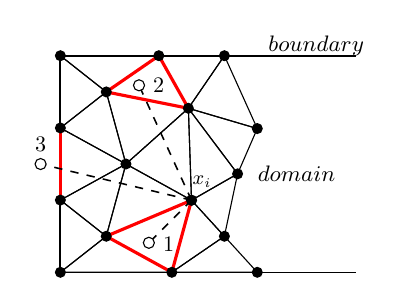
\begin{tikzpicture}[scale=2.5]

 % boundary 
 \draw[line width=0.2mm] (2.5,1.6) -- (4.0,1.6);
 \draw[line width=0.2mm] (2.5,1.6) -- (2.5,0.5);
 \draw[line width=0.2mm] (2.5,0.5) -- (4.0,0.5);

 % nodes
 \coordinate (A) at (2.500,0.5000) {};
 \coordinate (B) at (2.500,0.8667) {};
 \coordinate (C) at (2.500,1.2330) {};
 \coordinate (D) at (2.500,1.6000) {};
 \coordinate (E) at (2.733,0.6830) {};
 \coordinate (F) at (2.833,1.0500) {};
 \coordinate (G) at (2.733,1.4160) {};
 \coordinate (H) at (3.000,1.6000) {};
 \coordinate (I) at (3.066,0.5000) {};
 \coordinate (J) at (3.166,0.8660) {};
 \coordinate (K) at (3.150,1.3330) {};
 \coordinate (L) at (3.333,1.6000) {};
 \coordinate (M) at (3.500,0.5000) {};
 \coordinate (N) at (3.333,0.6830) {};
 \coordinate (O) at (3.400,1.0000) {};
 \coordinate (P) at (3.500,1.2300) {};

 % elements
 \draw (A) -- (E) -- (B) -- cycle;
 \draw (A) -- (I) -- (E) -- cycle;
 \draw (E) -- (J) -- (F) -- cycle;
 \draw (E) -- (F) -- (B) -- cycle;
 \draw (B) -- (F) -- (C) -- cycle;
 \draw (J) -- (K) -- (F) -- cycle;
 \draw (F) -- (K) -- (G) -- cycle;
 \draw (C) -- (F) -- (G) -- cycle;
 \draw (C) -- (G) -- (D) -- cycle;
 \draw (G) -- (H) -- (D) -- cycle;
 \draw (I) -- (N) -- (J) -- cycle;
 \draw (I) -- (M) -- (N) -- cycle;
 \draw (N) -- (O) -- (J) -- cycle;
 \draw (J) -- (O) -- (K) -- cycle;
 \draw (P) -- (L) -- (K) -- cycle;
 \draw (K) -- (L) -- (H) -- cycle;
 \draw (O) -- (P) -- (K) -- cycle;
 \draw[red,line width=0.04cm] (I) -- (J) -- (E) -- cycle;
 \draw[red,line width=0.04cm] (B) -- (C);
 \draw[red,line width=0.04cm] (G) -- (K) -- (H) -- cycle;
 

 % draw nodes
 \node[circle, fill=black, inner sep=0pt, minimum size=4pt] at (A) {};
 \node[circle, fill=black, inner sep=0pt, minimum size=4pt] at (B) {};
 \node[circle, fill=black, inner sep=0pt, minimum size=4pt] at (C) {};
 \node[circle, fill=black, inner sep=0pt, minimum size=4pt] at (D) {};
 \node[circle, fill=black, inner sep=0pt, minimum size=4pt] at (E) {};
 \node[circle, fill=black, inner sep=0pt, minimum size=4pt] at (F) {};
 \node[circle, fill=black, inner sep=0pt, minimum size=4pt] at (G) {};
 \node[circle, fill=black, inner sep=0pt, minimum size=4pt] at (H) {};
 \node[circle, fill=black, inner sep=0pt, minimum size=4pt] at (I) {};
 \node[circle, fill=black, inner sep=0pt, minimum size=4pt] at (J) {};
 \node[circle, fill=black, inner sep=0pt, minimum size=4pt] at (K) {};
 \node[circle, fill=black, inner sep=0pt, minimum size=4pt] at (L) {};
 \node[circle, fill=black, inner sep=0pt, minimum size=4pt] at (M) {};
 \node[circle, fill=black, inner sep=0pt, minimum size=4pt] at (N) {};
 \node[circle, fill=black, inner sep=0pt, minimum size=4pt] at (O) {};
 \node[circle, fill=black, inner sep=0pt, minimum size=4pt] at (P) {};


 % arrow
 \draw[dashed,line width=0.02cm] (J) edge (2.95,0.65);
 \draw[dashed,line width=0.02cm] (J) edge (2.90,1.45);
 \draw[dashed,line width=0.02cm] (J) edge (2.4,1.05) ;

 \node[circle, fill=black, inner sep=0pt, minimum size=4pt] at (J) {};

 % departure nodes
 \node[circle, fill=white, draw, inner sep=0pt, minimum size=4pt] at (2.95,0.65) {};
 \node[circle, fill=white, draw, inner sep=0pt, minimum size=4pt] at (2.90,1.45) {};
 \node[circle, fill=white, draw, inner sep=0pt, minimum size=4pt] at (2.4,1.05) {};


 
 % legend
 \node[draw=none, scale=0.8] at (3.22,0.96) {\small $x_{i}$};
 
 \node[draw=none, scale=0.8] at (3.05,0.64) {$1$};
 \node[draw=none, scale=0.8] at (3.00,1.45) {$2$};
 \node[draw=none, scale=0.8] at (2.4,1.15) {$3$};
 
 \node[draw=none, scale=0.9] at (3.7,1.0) {\small $domain$};
 \node[draw=none, scale=0.9] at (3.8,1.65) {\small $boundary$};
\end{tikzpicture}
\end{center}
\end{columns}


\vspace{0.6cm}
\justifying
\tiny [3]
Pironneau, O. On the transport-diffusion algorithm and its applications to the Navier-Stokes equations. Numer. Math. 38, 309–332 (1982). \textit{https://doi.org/10.1007/BF01396435}
\end{frame}



%%%%%%%%%%%%%%%%%%%%%%%%%%%%%%%%%%%%%%%%%%%%%%%%%%%%%%%%%%%%%%%%%%%%%%%%%%%%%%%%%%%%%%%%%%



\begin{frame} 
 \frametitle{\LARGE Galerkin FE Method}
\vspace{-1.2cm}
\begin{columns}[c]
\column{.5\textwidth}
\begin{figure}[H]
\begin{center}
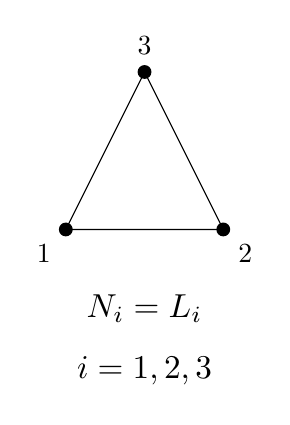
\begin{tikzpicture}[scale=2]
 \draw (0,0) -- (1,0) -- (0.5,1) -- cycle;

 \node[circle, fill=black, inner sep=0pt, minimum size=5pt,label=below left:{1}] at (0,0) {};
 \node[circle, fill=black, inner sep=0pt, minimum size=5pt,label=below right:{2}] at (1,0) {};
 \node[circle, fill=black, inner sep=0pt, minimum size=5pt,label=above:{3}] at (0.5,1) {};
 
 \node[draw=none, scale=1.2] at (0.5,-0.5) {$N_i = L_i$};
 \node[draw=none, scale=1.2] at (0.5,-0.9) {$i = 1,2,3$};
\end{tikzpicture}
\end{center}
\end{figure}

\vspace{-1cm}
\column{.5\textwidth}
\begin{center}
\begin{equation*}
 \left[ \frac{\mathbf{M}}{\Delta t} + \frac{\mathbf{K}}{Re} \right] \omega_{i}^{n+1} = \frac{\mathbf{M}}{\Delta t} \omega_{d}^{n}
\end{equation*}
\medskip
\begin{equation*}
 \mathbf{K} \psi = \mathbf{M} \omega
\end{equation*}
\medskip
\begin{equation*}
 \left[ \frac{\mathbf{M}}{\Delta t} + \frac{\mathbf{K}}{ReSc} \right] c_{i}^{n+1} = \frac{\mathbf{M}}{\Delta t} c_{d}^{n}
\end{equation*}
\end{center}
\end{columns}

\vspace{1.2cm}
\justifying
The material velocity field is calculated by: 
$\mathbf{M} v_{x} = \mathbf{G_{y}} \psi$ and 
$\mathbf{M} v_{y} = - \mathbf{G_{x}} \psi$



\end{frame}

%%%%%%%%%%%%%%%%%%%%%%%%%%%%%%%%%%%%%%%%%%%%%%%%%%%%%%%%%%%%%%%%%%%%%%%%%%%%%%%%%%%%%%%%%%

\begin{frame}
 \frametitle{\LARGE Adaptive Mesh Refinement}
 Laplace Smoothing description, comparative figures and ALE velocity formula
\end{frame}


%%%%%%%%%%%%%%%%%%%%%%%%%%%%%%%%%%%%%%%%%%%%%%%%%%%%%%%%%%%%%%%%%%%%%%%%%%%%%%%%%%%%%%%%%%

\begin{frame} 
 \frametitle{\LARGE Solution Algorithm}
\vspace{-1cm}
% Define block styles
\tikzstyle{block} = [rectangle, draw,
    text width=27em, text centered, rounded corners, fill=gray!45!,scale=0.75,text=black!90!]
\tikzstyle{line} = [draw, -latex',scale=0.75]

\begin{center}
\begin{tikzpicture}[node distance = 1cm, auto]
    % Place nodes
    \node [block] (step1) {inicialize vorticity};
    \node [block, below of=step1] (step2) {inicialize stream function};
    \node [block, below of=step2] (step3) {Calculate vorticity boundary condition};
    \node [block, below of=step3] (step4) {Calculate vorticity};
    \node [block, below of=step4] (step5) {Calculate stream function};
    \node [block, below of=step5] (step6) {Calculate velocity};
    \node [block, below of=step6] (step7) {Calculate concentration};
    \node [draw=none, align=center,scale=0.7,text=black!80!] at (6,-3) {Repeat the procedure \\ for the next time step};
    % Draw edges
    \path [line] (step1) -- (step2);
    \path [line] (step2) -- (step3);
    \path [line] (step3) -- (step4);
    \path [line] (step4) -- (step5);
    \path [line] (step5) -- (step6);
    \path [line] (step6) -- (step7);
    \path [line,dashed] (step7) -- (6,-6) |- (step3);
\end{tikzpicture}
\end{center}
\vspace{0.5cm}
\centering \scriptsize Streamfunction-Vorticity formulation with species transport equation solution algorithm

\end{frame}

%%%%%%%%%%%%%%%%%%%%%%%%%%%%%%%%%%%%%%%%%%%%%%%%%%%%%%%%%%%%%%%%%%%%%%%%%%%%%%%%%%%%%%%%%%

\begin{frame}
  \vspace{-1cm}
  \textcolor{gray}{1. Introduction}\\[0.1cm]
  \textcolor{gray}{2. Mathematical Model}\\[0.1cm]
  3. Validation\\[0.1cm]
  \textcolor{gray}{4. Results}\\[0.1cm]
  \textcolor{gray}{5. Conclusion}
\end{frame}


%%%%%%%%%%%%%%%%%%%%%%%%%%%%%%%%%%%%%%%%%%%%%%%%%%%%%%%%%%%%%%%%%%%%%%%%%%%%%%%%%%%%%%%%%%
\iffalse
\begin{frame}
 \frametitle{\small Validation - Poiseuille Flow}
\vspace{-0.7cm}
\begin{center}
\begin{columns}[c]
\begin{column}{0.55\textwidth} 
\small
Boundaries Conditions:\\[0.2cm]
Inflow condition: $u=1$, $v=0$ e $\psi=y$\\[0.1cm]
Outflow condition: $\psi=y$\\[0.1cm]
Top plate: $u=0$, $v=0$, $\psi=1$\\[0.1cm]
Bottom plate: $u=0$, $v=0$, $\psi=0$
\end{column}
\begin{column}{0.35\textwidth} 
\begin{tikzpicture}[scale=0.8]
 \draw [pattern=north east lines] (0,0) -- (0,-0.1) -- (5,-0.1) -- (5,0) -- cycle;
 \draw [pattern=north east lines] (0,1) -- (0,1.1) -- (5,1.1) -- (5,1) -- cycle;
 \draw [dotted] (0,0.9) -- (5,0.9);
 \draw [dotted] (0,0.7) -- (5,0.7);
 \draw [dotted] (0,0.5) -- (5,0.5);
 \draw [dotted] (0,0.3) -- (5,0.3);
 \draw [dotted] (0,0.1) -- (5,0.1);

% \draw [->,thick] (-2,-0.1)--(-2,1.5) node[left] {$y$};
% \draw [->,thick] (-2.1,0)--(-0.5,0) node[below] {$x$};

 \draw  (4.0,0.0) to [bend right=100] (4.0,1.0);
 \draw  (2.5,0.0) to [bend right=100] (2.5,1.0);
 \draw  (1.0,0.0) to [bend right=100] (1.0,1.0);

 \draw [->,thick] (4.0,0.9) to (4.2,0.9);
 \draw [->,thick] (4.0,0.7) to (4.28,0.7);
 \draw [->,thick] (4.0,0.5) to (4.3,0.5);
 \draw [->,thick] (4.0,0.3) to (4.28,0.3);
 \draw [->,thick] (4.0,0.1) to (4.2,0.1);

 \draw [->,thick] (2.5,0.9) to (2.7,0.9);
 \draw [->,thick] (2.5,0.7) to (2.78,0.7);
 \draw [->,thick] (2.5,0.5) to (2.8,0.5);
 \draw [->,thick] (2.5,0.3) to (2.78,0.3);
 \draw [->,thick] (2.5,0.1) to (2.7,0.1);

 \draw [->,thick] (1.0,0.9) to (1.2,0.9);
 \draw [->,thick] (1.0,0.7) to (1.28,0.7);
 \draw [->,thick] (1.0,0.5) to (1.3,0.5);
 \draw [->,thick] (1.0,0.3) to (1.28,0.3);
 \draw [->,thick] (1.0,0.1) to (1.2,0.1);
\end{tikzpicture}
\end{column}
\end{columns}
\end{center}
\vspace{-0.5cm}
\begin{center}
\begin{columns}[c]
\begin{column}{0.4\textwidth} 
\begin{equation*}
u = \frac{4 u_{max}}{L^2} y \big[ L - y \big]
\end{equation*}
\end{column}
\begin{column}{0.73\textwidth} 
\begin{figure}
  \centering
  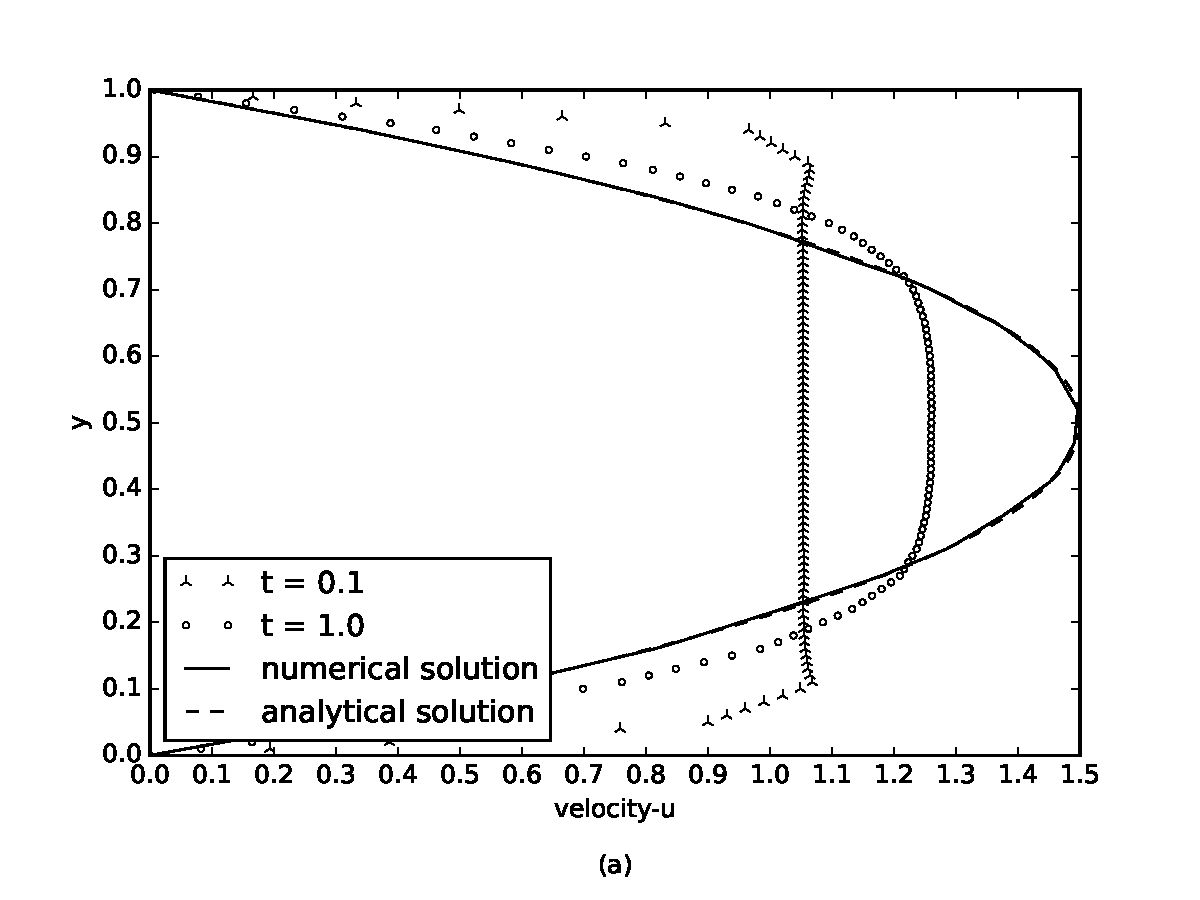
\includegraphics[scale=0.48]{images/poiseuille_velocity.pdf}
\end{figure}
%\vspace{-0.2cm}
%\centering \scriptsize Evolution of velocity field profile in time for \textit{$Re = 100$} and the comparison between numerical solution and analytical solution
\end{column}
\end{columns}
\end{center}
\end{frame}
\fi


%%%%%%%%%%%%%%%%%%%%%%%%%%%%%%%%%%%%%%%%%%%%%%%%%%%%%%%%%%%%%%%%%%%%%%%%%%%%%%%%%%%%%%%%%%

\begin{frame}
 \frametitle{\LARGE Validation - Poiseuille Flow}
\vspace{-0.55cm}
\begin{center}
\begin{columns}[c]
\begin{column}{0.55\textwidth} 
\small
Boundaries Conditions:\\[0.2cm]
Inflow condition: $u=1$, $v=0$ e $\psi=y$\\[0.1cm]
Outflow condition: $\psi=y$\\[0.1cm]
Top plate: $u=0$, $v=0$, $\psi=1$\\[0.1cm]
Bottom plate: $u=0$, $v=0$, $\psi=0$
\end{column}
\begin{column}{0.35\textwidth} 
\begin{tikzpicture}[scale=0.8]
 \draw [pattern=north east lines] (0,0) -- (0,-0.1) -- (5,-0.1) -- (5,0) -- cycle;
 \draw [pattern=north east lines] (0,1) -- (0,1.1) -- (5,1.1) -- (5,1) -- cycle;
 \draw [dotted] (0,0.9) -- (5,0.9);
 \draw [dotted] (0,0.7) -- (5,0.7);
 \draw [dotted] (0,0.5) -- (5,0.5);
 \draw [dotted] (0,0.3) -- (5,0.3);
 \draw [dotted] (0,0.1) -- (5,0.1);

% \draw [->,thick] (-2,-0.1)--(-2,1.5) node[left] {$y$};
% \draw [->,thick] (-2.1,0)--(-0.5,0) node[below] {$x$};

 \draw  (4.0,0.0) to [bend right=100] (4.0,1.0);
 \draw  (2.5,0.0) to [bend right=100] (2.5,1.0);
 \draw  (1.0,0.0) to [bend right=100] (1.0,1.0);

 \draw [->,thick] (4.0,0.9) to (4.2,0.9);
 \draw [->,thick] (4.0,0.7) to (4.28,0.7);
 \draw [->,thick] (4.0,0.5) to (4.3,0.5);
 \draw [->,thick] (4.0,0.3) to (4.28,0.3);
 \draw [->,thick] (4.0,0.1) to (4.2,0.1);

 \draw [->,thick] (2.5,0.9) to (2.7,0.9);
 \draw [->,thick] (2.5,0.7) to (2.78,0.7);
 \draw [->,thick] (2.5,0.5) to (2.8,0.5);
 \draw [->,thick] (2.5,0.3) to (2.78,0.3);
 \draw [->,thick] (2.5,0.1) to (2.7,0.1);

 \draw [->,thick] (1.0,0.9) to (1.2,0.9);
 \draw [->,thick] (1.0,0.7) to (1.28,0.7);
 \draw [->,thick] (1.0,0.5) to (1.3,0.5);
 \draw [->,thick] (1.0,0.3) to (1.28,0.3);
 \draw [->,thick] (1.0,0.1) to (1.2,0.1);
\end{tikzpicture}
\end{column}
\end{columns}
\end{center}
\vspace{-1.0cm}
\begin{center}
\begin{columns}[c]
\begin{column}{0.55\textwidth} 
\begin{figure}
  \centering
  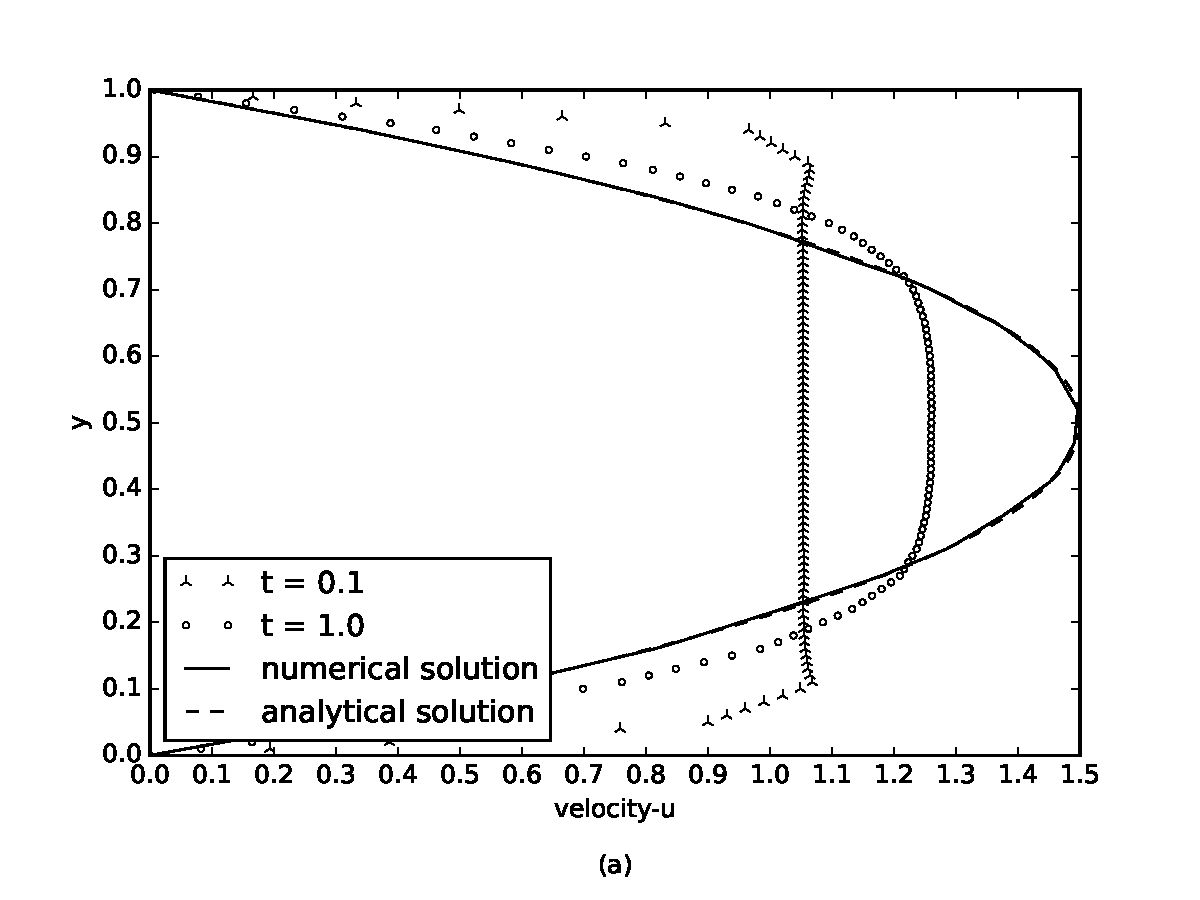
\includegraphics[scale=0.33]{images/poiseuille_velocity.pdf}
\end{figure}
\end{column}
\begin{column}{0.65\textwidth} 
\begin{figure}
  \centering
  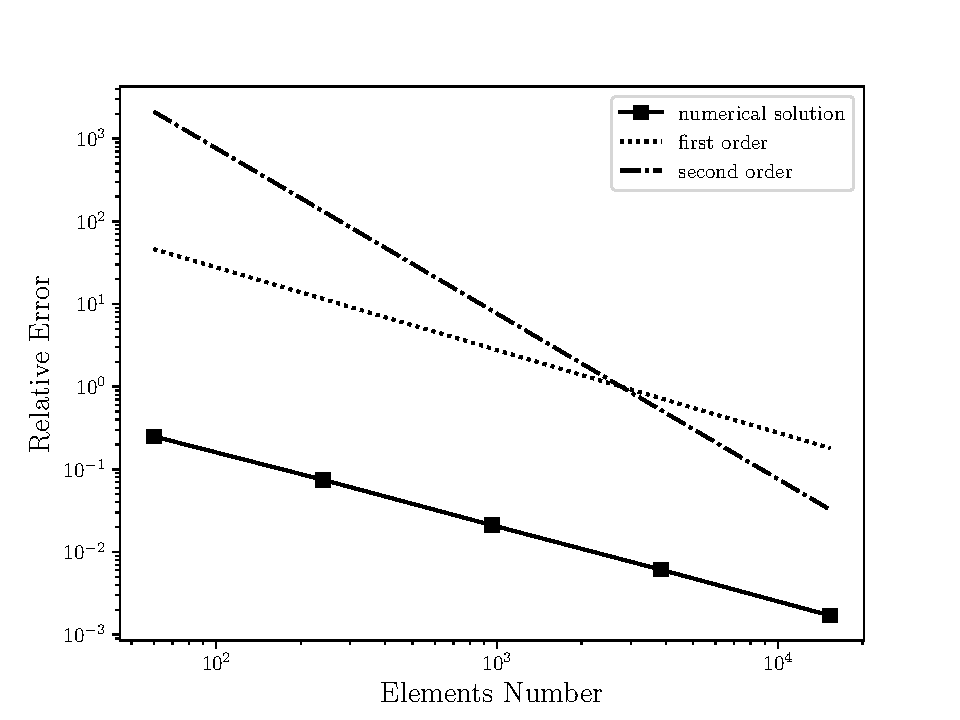
\includegraphics[scale=0.33]{images/poiseuille_error.pdf}
\end{figure}
\end{column}
\end{columns}
\vspace{0.06cm}
\centering \scriptsize (a) comparison of Poiseuille Flow velocity profile and\\ (b) log scale graph of convergence order.
\end{center}
\end{frame}





%%%%%%%%%%%%%%%%%%%%%%%%%%%%%%%%%%%%%%%%%%%%%%%%%%%%%%%%%%%%%%%%%%%%%%%%%%%%%%%%%%%%%%%%%%


\iffalse
\begin{frame}
 \frametitle{\small Validation - Poiseuille Flow}
\begin{figure}
  \centering
  \vspace{-1.5cm}
  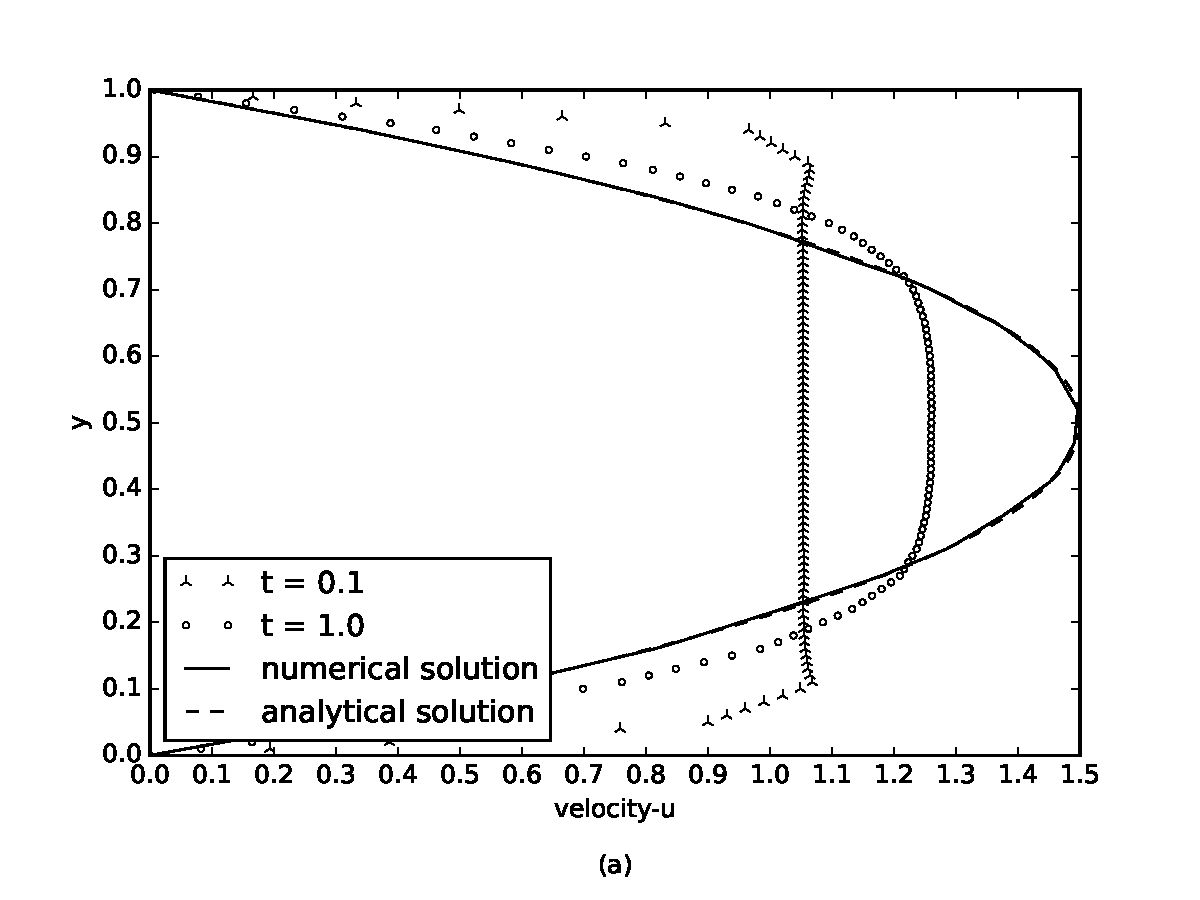
\includegraphics[scale=0.6]{images/poiseuille_velocity.pdf}
\end{figure}
\vspace{-0.2cm}
\centering \scriptsize Evolution of velocity field profile in time for \textit{$Re = 100$} and the comparison between numerical solution and analytical solution.
\end{frame}
\fi

%%%%%%%%%%%%%%%%%%%%%%%%%%%%%%%%%%%%%%%%%%%%%%%%%%%%%%%%%%%%%%%%%%%%%%%%%%%%%%%%%%%%%%%%%%

\begin{frame}
 \frametitle{\LARGE Validation - Lid Driven Cavity Flow}
\vspace{-1.1cm}
\begin{center}
\begin{columns}[c]
\begin{column}{0.65\textwidth} 
\small
Boundaries Conditions:\\[0.2cm]
Bottom and side plates: $u=0$, $v=0$ e $\psi=0$\\[0.1cm]
Top plate: $u=1$, $v=0$ e $\psi=0$
\end{column}
\begin{column}{0.25\textwidth} 
\begin{tikzpicture}[scale=0.6]
\draw [pattern=north east lines] (0,-0.1) -- (3,-0.1) -- (3,3) -- (2.9,3) -- (2.9,0) -- (0.1,0) -- (0.1,3) -- (0,3) -- cycle;
 \draw [pattern=north east lines] (-0.1,3) -- (-0.1,3.1) -- (3.1,3.1) -- (3.1,3) -- cycle;

 \draw [->,thick] (3.2,3.05)--(4.2,3.05) node[above] {$U_{top}$};

 \draw [->,thick] (2.4,2.4) arc (45:-180:1.2);

% \draw [->,thick] (-2,-0.1)--(-2,1.5) node[left] {$y$};
% \draw [->,thick] (-2.1,0)--(-0.5,0) node[below] {$x$};
\end{tikzpicture}
\end{column}
\end{columns}
\end{center}
\vspace{-0.6cm}
\begin{center}
\begin{columns}[c]
\begin{column}{0.55\textwidth} 
\begin{figure}
  \centering
  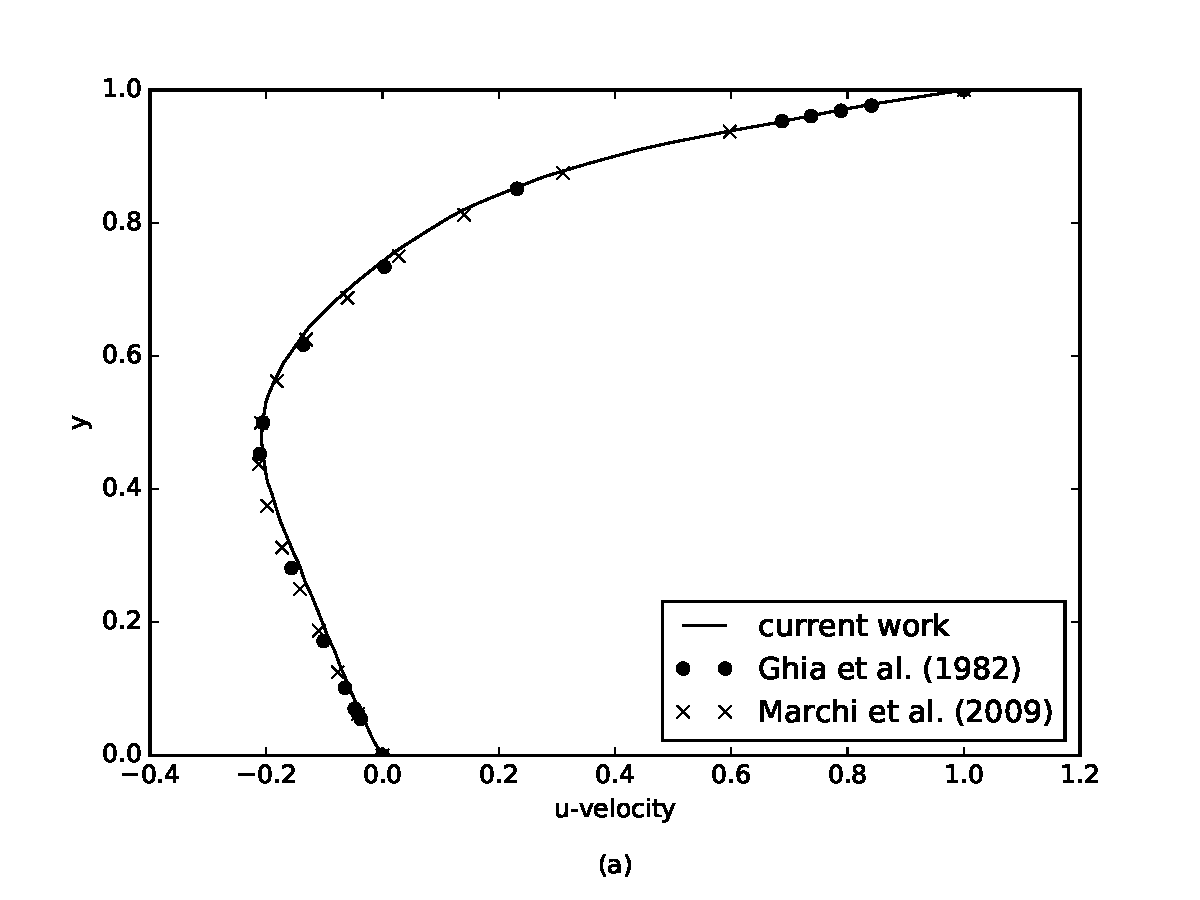
\includegraphics[scale=0.33]{images/Re_100_u_profile.pdf}
\end{figure}
\end{column}
\begin{column}{0.65\textwidth} 
\begin{figure}
  \centering
  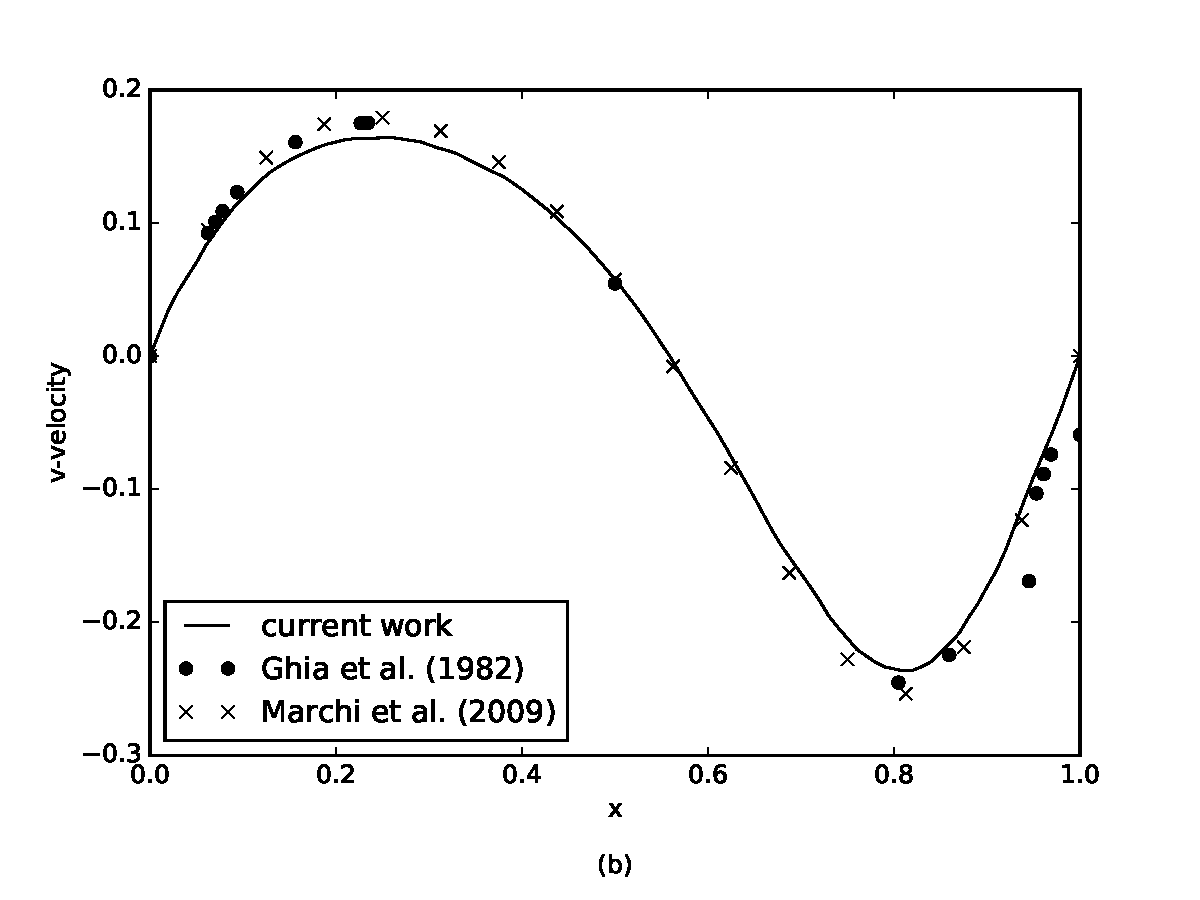
\includegraphics[scale=0.33]{images/Re_100_v_profile.pdf}
\end{figure}
\end{column}
\end{columns}
\vspace{0.1cm}
\centering \scriptsize Centerline velocity profile in a lid-driven cavity for $Re=100$: \\ (a) u-velocity and (b) v-velocity.
\end{center}
\end{frame}



%%%%%%%%%%%%%%%%%%%%%%%%%%%%%%%%%%%%%%%%%%%%%%%%%%%%%%%%%%%%%%%%%%%%%%%%%%%%%%%%%%%%%%%%%%

\iffalse
\begin{frame}
 \frametitle{\small Validation - Lid Driven Cavity Flow}
\vspace{-1cm}
\begin{center}
\begin{tikzpicture}[scale=0.8]
\draw [pattern=north east lines] (0,-0.1) -- (3,-0.1) -- (3,3) -- (2.9,3) -- (2.9,0) -- (0.1,0) -- (0.1,3) -- (0,3) -- cycle;
 \draw [pattern=north east lines] (-0.1,3) -- (-0.1,3.1) -- (3.1,3.1) -- (3.1,3) -- cycle;

 \draw [->,thick] (3.2,3.05)--(4.2,3.05) node[above] {$U_{top}$};

 \draw [->,thick] (2.4,2.4) arc (45:-180:1.2);

% \draw [->,thick] (-2,-0.1)--(-2,1.5) node[left] {$y$};
% \draw [->,thick] (-2.1,0)--(-0.5,0) node[below] {$x$};
\end{tikzpicture}
\end{center}
\vspace{0.5cm}
\small
Boundaries Conditions:\\[0.2cm]
Bottom and side plates: $u=0$, $v=0$ e $\psi=0$;\\[0.1cm]
Top plate: $u=1$, $v=0$ e $\psi=0$
\end{frame}
\fi

%%%%%%%%%%%%%%%%%%%%%%%%%%%%%%%%%%%%%%%%%%%%%%%%%%%%%%%%%%%%%%%%%%%%%%%%%%%%%%%%%%%%%%%%%%

\iffalse
\begin{frame}
 \frametitle{\small Validation - Lid Driven Cavity Flow}
\begin{figure}
  \centering
  \vspace{-1.5cm}
  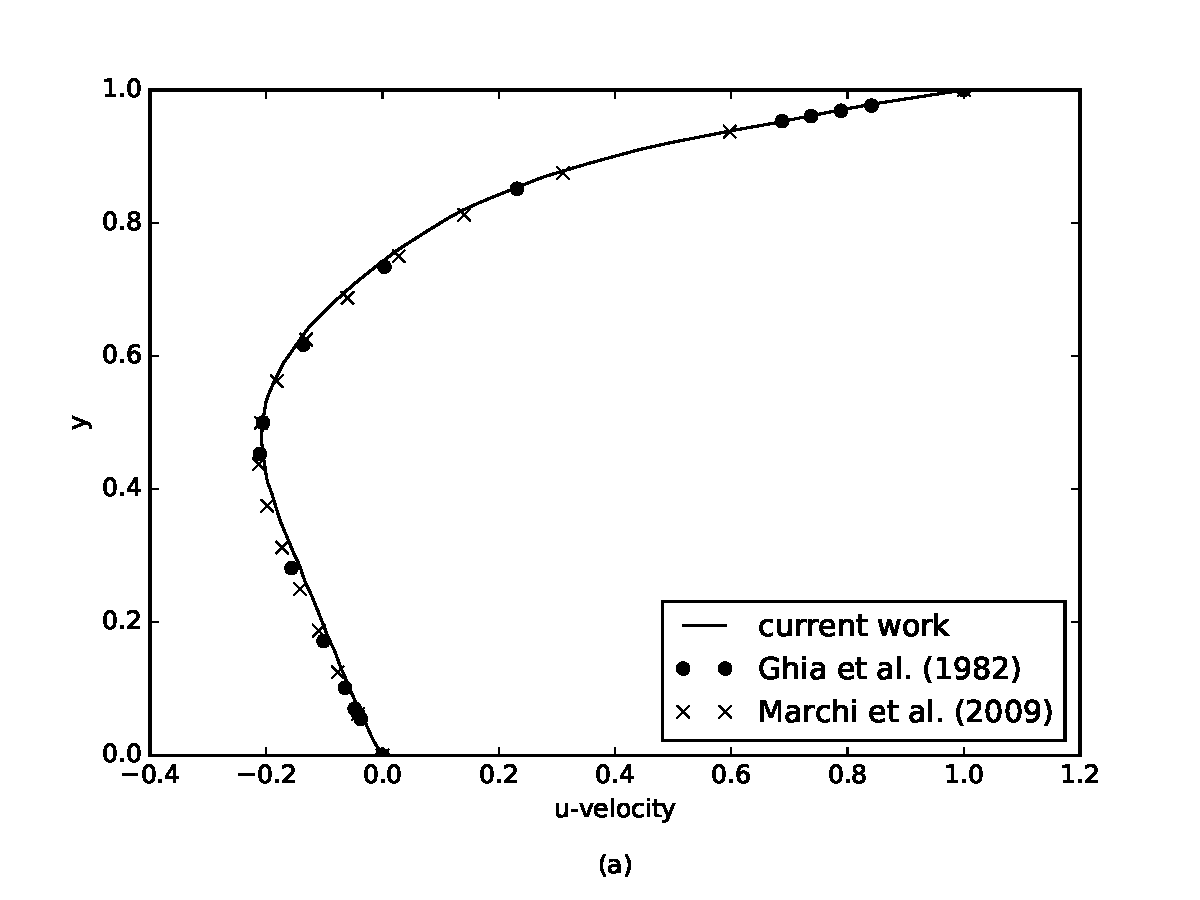
\includegraphics[scale=0.6]{images/Re_100_u_profile.pdf}
\end{figure}
\vspace{-0.2cm}
\centering \scriptsize Centerline $u$ velocity profile ($x=0.5$) in a lid-driven cavity for $Re=100$.
\end{frame}
\fi

%%%%%%%%%%%%%%%%%%%%%%%%%%%%%%%%%%%%%%%%%%%%%%%%%%%%%%%%%%%%%%%%%%%%%%%%%%%%%%%%%%%%%%%%%%
\iffalse
\begin{frame}
 \frametitle{\small Validation - Lid Driven Cavity Flow}
\begin{figure}
  \centering
  \vspace{-1.5cm}
  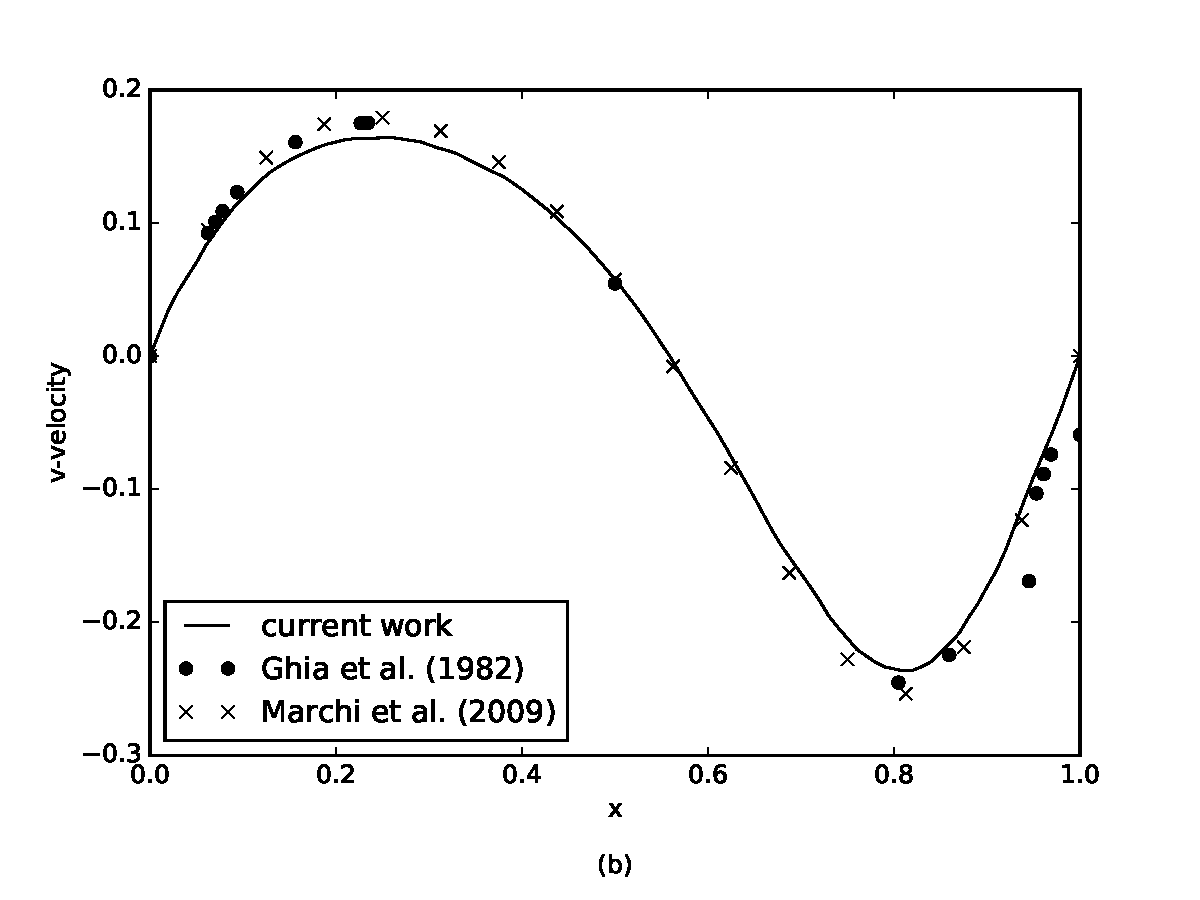
\includegraphics[scale=0.6]{images/Re_100_v_profile.pdf}
\end{figure}
\vspace{-0.2cm}
\centering \scriptsize Centerline $v$ velocity profile ($y=0.5$) in a lid-driven cavity for $Re=100$.
\end{frame}
\fi

%%%%%%%%%%%%%%%%%%%%%%%%%%%%%%%%%%%%%%%%%%%%%%%%%%%%%%%%%%%%%%%%%%%%%%%%%%%%%%%%%%%%%%%%%%

\begin{frame}
  \vspace{-1cm}
  \textcolor{gray}{1. Introduction}\\[0.1cm]
  \textcolor{gray}{2. Mathematical Model}\\[0.1cm]
  \textcolor{gray}{3. Validation}\\[0.1cm]
  4. Results\\[0.1cm]
  \textcolor{gray}{5. Conclusion}
\end{frame}


%%%%%%%%%%%%%%%%%%%%%%%%%%%%%%%%%%%%%%%%%%%%%%%%%%%%%%%%%%%%%%%%%%%%%%%%%%%%%%%%%%%%%%%%%%

\begin{frame}
 \frametitle{\LARGE Results}
\begin{figure}
  \vspace{-1cm}
     \centering
     \begin{minipage}{.45\linewidth}
      \centering
      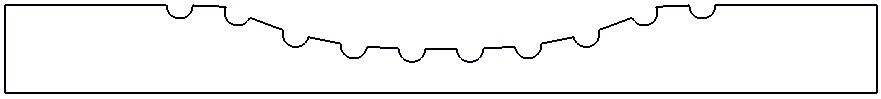
\includegraphics[scale=0.15]{images/CurvedStrut.png}\\
      \scriptsize (a)
     \end{minipage}%
     \begin{minipage}{.45\linewidth}
      \centering
      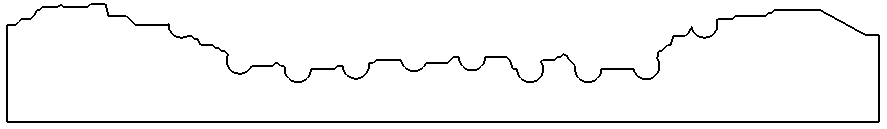
\includegraphics[scale=0.15]{images/RealStrut.png}\\
      \scriptsize (b)
     \end{minipage}
\end{figure}
\vspace{-0.3cm}
\begin{center}
\scriptsize 
     Non-dimensional symmetric geometry for blood flow in coronary artery with drug-eluting stent placed by Wang et al. (2017):
     (a) Curved Channel with Stent
     (b) Real Channel with Stent.
\end{center}
\vspace{0.05cm}
\small
\begin{center}
\begin{columns}[c]
\begin{column}{0.8\textwidth} 
Boundaries Conditions:\\[0.2cm]
Inflow condition: $u=1$, $v=0$ e $\psi=y$;\\[0.1cm]
Outflow condition: $\psi=y$;\\[0.1cm]
Top plate: $u=0$, $v=0$, $\psi=1$;\\[0.1cm]
Symmetry condition: $v=0$, $\psi=0$; \\[0.1cm]
Drug-eluting stent: $u=0$, $v=0$, $\psi=1$ e $c=1$
\end{column}
\hspace{-1cm}
\begin{column}{0.3\textwidth}
$R=0.0015m$\\[0.1cm]
$\mu=0.0035Pa.s$\\[0.1cm]
$\rho=1060kg/m^3$\\[0.1cm]\\
$u=12cm/s$\\[0.1cm]
$Re=54.5$
\end{column}
\end{columns}
\end{center}
\end{frame}


%%%%%%%%%%%%%%%%%%%%%%%%%%%%%%%%%%%%%%%%%%%%%%%%%%%%%%%%%%%%%%%%%%%%%%%%%%%%%%%%%%%%%%%%%%

\iffalse
\begin{frame}
 \frametitle{\LARGE Results}
\begin{figure}
     \begin{minipage}{.50\linewidth}
      \centering
      
\includegraphics[scale=0.08]{images/vel_RealStrut200.png}\\
      \scriptsize t = 0.1
     \end{minipage}%
     \begin{minipage}{.50\linewidth}
      \centering
      
\includegraphics[scale=0.08]{images/vel_RealStrut1000.png}\\
      \scriptsize t = 0.5
     \end{minipage}
     \begin{minipage}{.50\linewidth}
     \medskip
      \centering
      
\includegraphics[scale=0.08]{images/vel_RealStrut2000.png}\\
      \scriptsize t = 1.0
     \end{minipage}%
     \begin{minipage}{.50\linewidth}
     \medskip
      \centering
      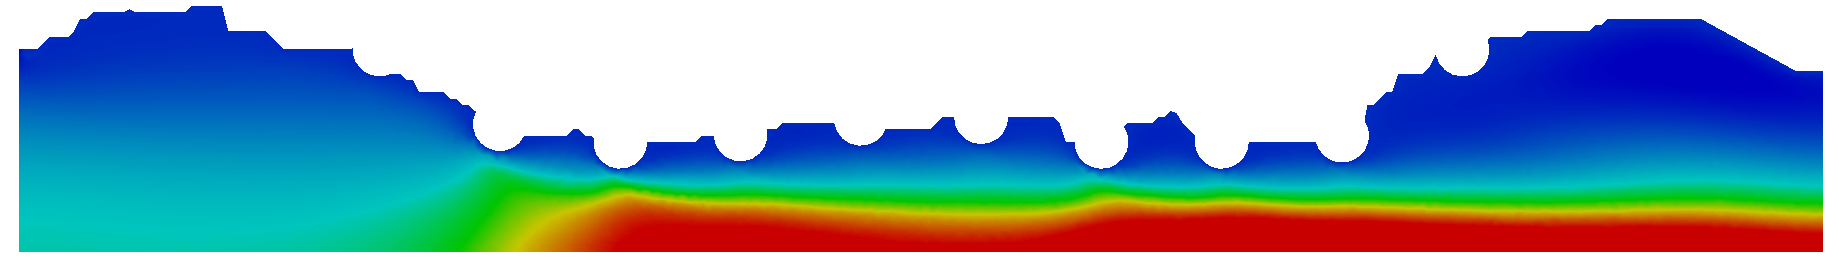
\includegraphics[scale=0.08]{images/vel_RealStrut6000.png}\\
      \scriptsize t = 3.0
     \end{minipage}
     \begin{minipage}{.50\linewidth}
      \centering
      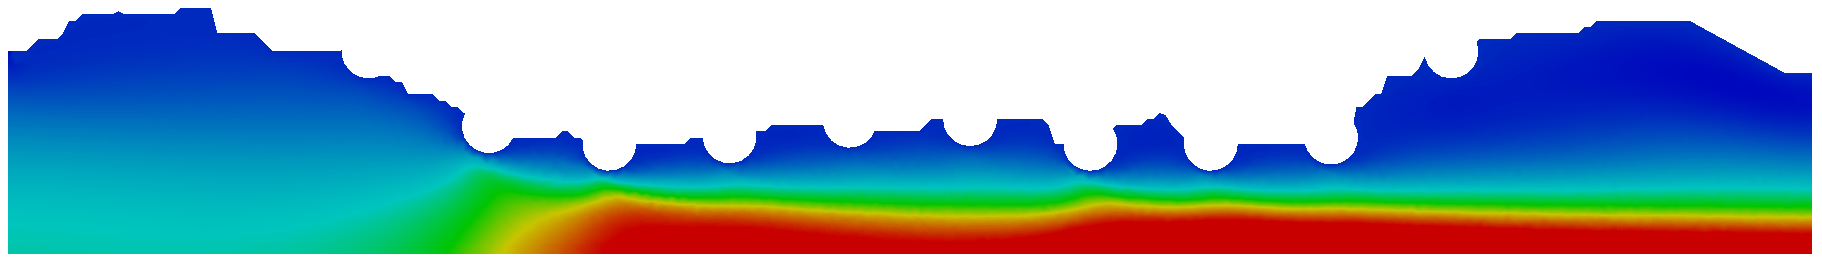
\includegraphics[scale=0.08]{images/vel_RealStrut8000.png}\\
      \scriptsize t = 4.0
     \end{minipage}%
     \begin{minipage}{.50\linewidth}
      \centering
      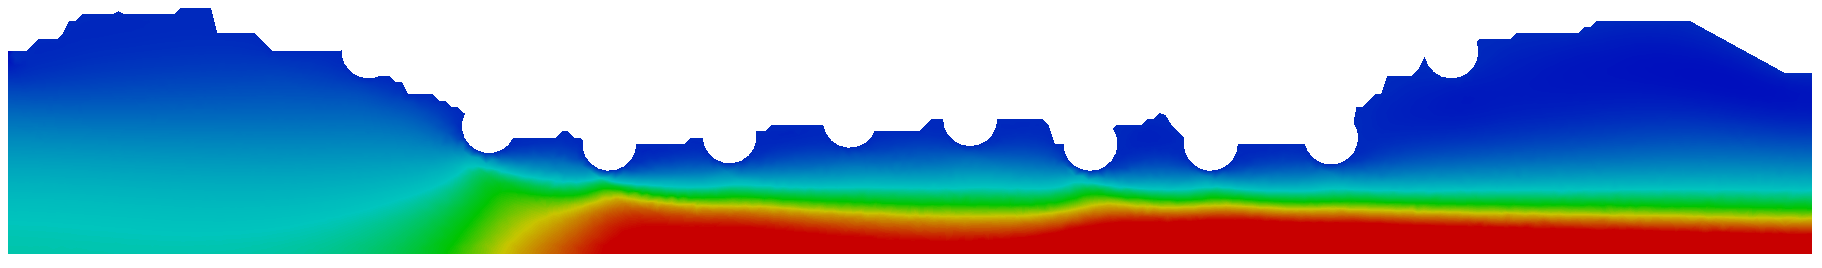
\includegraphics[scale=0.08]{images/vel_RealStrut10000.png}\\
      \scriptsize t = 5.0
 \end{minipage}
     \begin{minipage}{.50\linewidth}
     \medskip
      \centering
      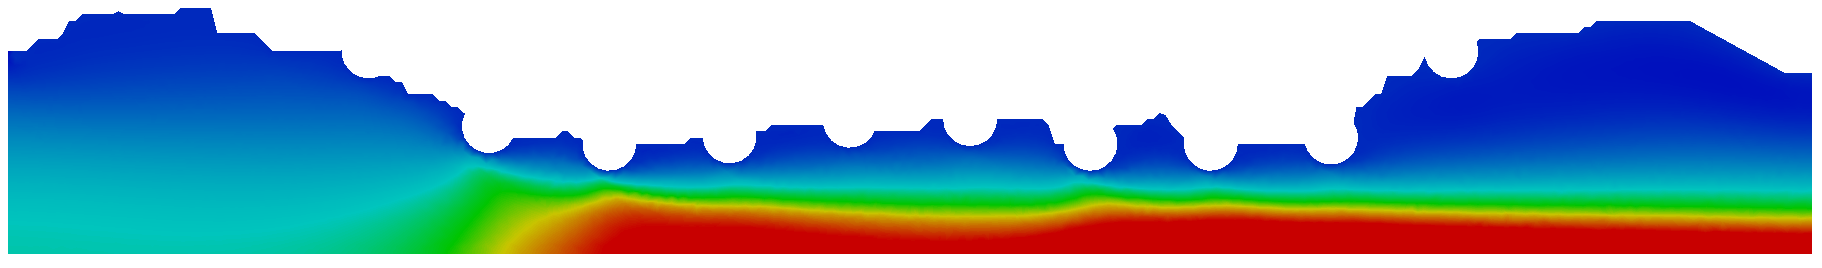
\includegraphics[scale=0.08]{images/vel_RealStrut14000.png}\\
      \scriptsize t = 7.0
     \end{minipage}%
     \begin{minipage}{.50\linewidth}
     \medskip
      \centering
      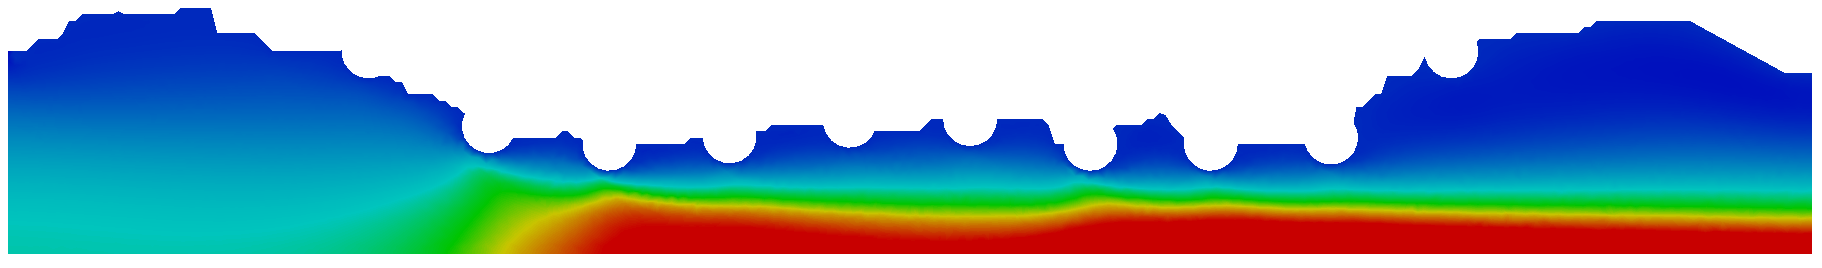
\includegraphics[scale=0.08]{images/vel_RealStrut20000.png}\\
      \scriptsize t = 10.0
     \end{minipage}
\end{figure}
\vspace{0cm}
\centering \scriptsize Evolution in time and space of velocity field
\end{frame}
\fi

%%%%%%%%%%%%%%%%%%%%%%%%%%%%%%%%%%%%%%%%%%%%%%%%%%%%%%%%%%%%%%%%%%%%%%%%%%%%%%%%%%%%%%%%%%

\begin{frame}
 \frametitle{\LARGE Results - Velocity Field}

\vspace{-0.8cm}
\begin{figure}
     \begin{minipage}{.50\linewidth}
      \centering
      
\includegraphics[scale=0.075]{images/vel_CurvedStrut2000.png}\\
      \tiny t = 1.0
     \end{minipage}%
     \begin{minipage}{.50\linewidth}
      \centering
      
\includegraphics[scale=0.075]{images/vel_RealStrut2000.png}\\
      \tiny t = 1.0
     \end{minipage}
     \begin{minipage}{.50\linewidth}
     \smallskip
      \centering
      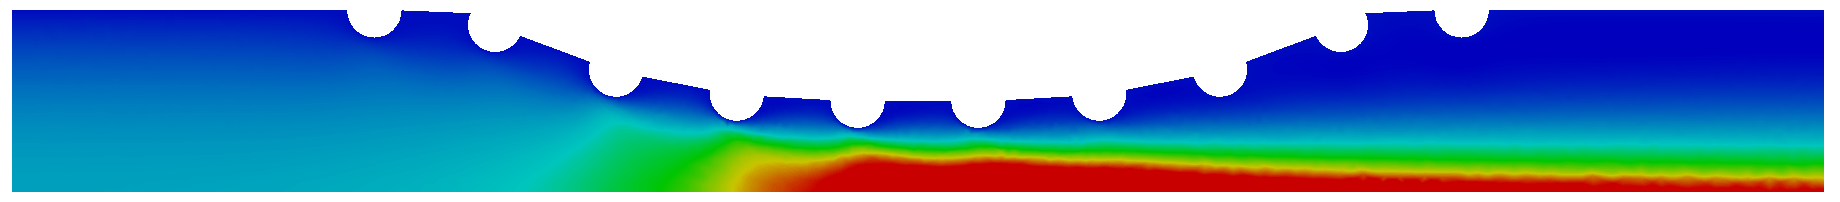
\includegraphics[scale=0.075]{images/vel_CurvedStrut10000.png}\\
      \tiny t = 5.0
     \end{minipage}%
     \begin{minipage}{.50\linewidth}
     \smallskip
      \centering
      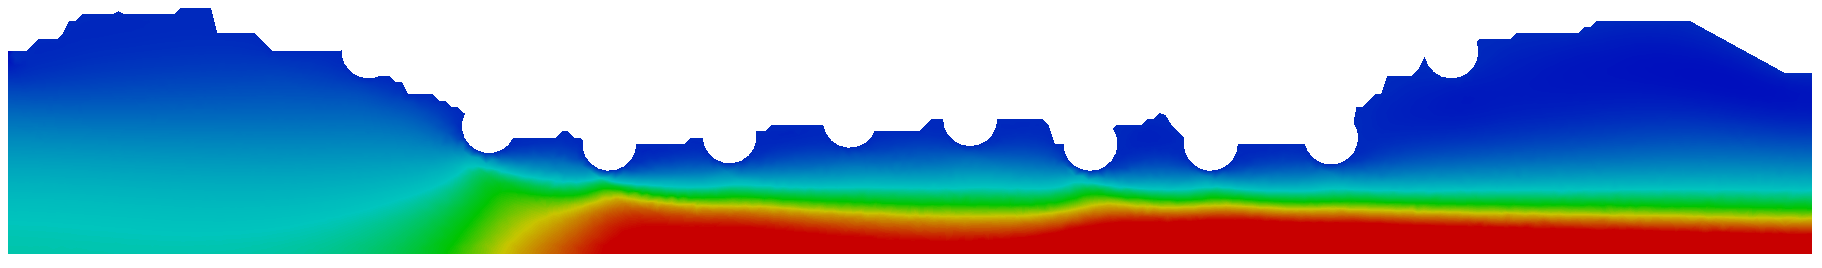
\includegraphics[scale=0.075]{images/vel_RealStrut10000.png}\\
      \tiny t = 5.0
     \end{minipage}
     \begin{minipage}{.50\linewidth}
      \centering
      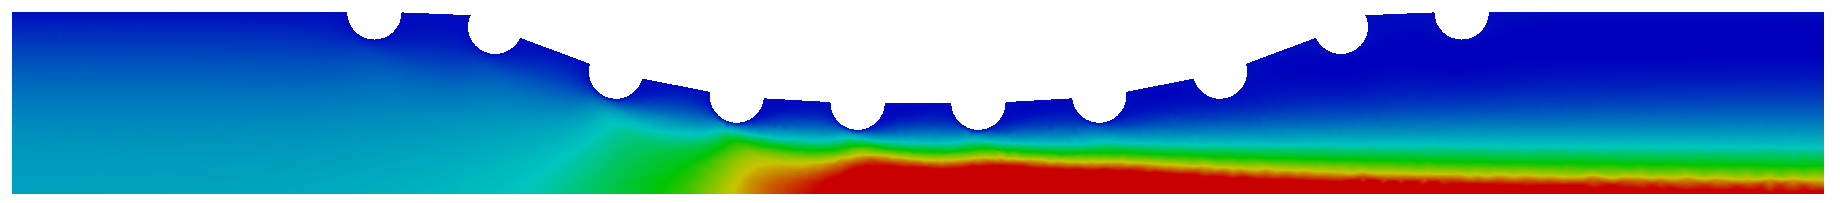
\includegraphics[scale=0.075]{images/vel_CurvedStrut20000.png}\\
      \tiny t = 10.0
     \end{minipage}%
     \begin{minipage}{.50\linewidth}
      \centering
      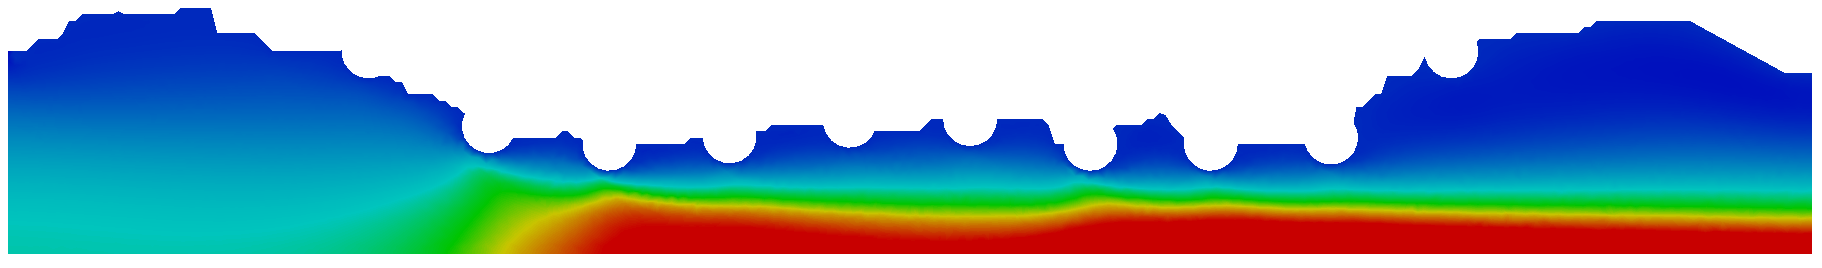
\includegraphics[scale=0.075]{images/vel_RealStrut20000.png}\\
      \tiny t = 10.0
     \end{minipage}
\end{figure}
\vspace{-0.2cm}
\centering \tiny Evolution in time and space of velocity field:\\
                 Curved Channel (left column) and Real Channel (right column)
\vspace{-0.5cm}
\begin{figure}
     \begin{minipage}{.50\linewidth}
     \medskip
      \centering
      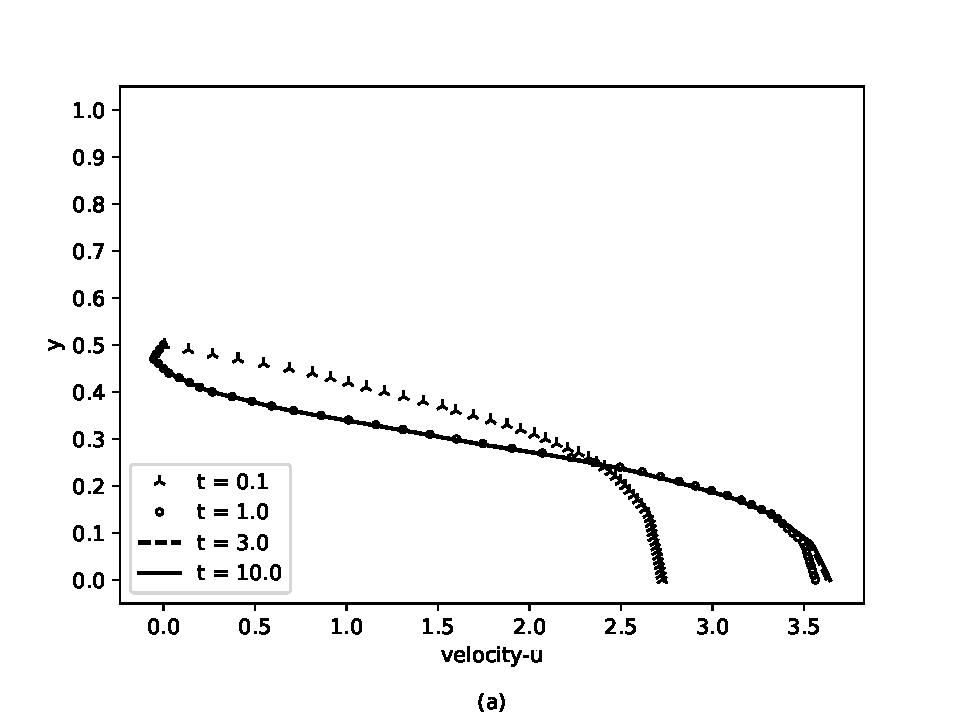
\includegraphics[scale=0.35]{images/vel_CurvedStrut_evol.pdf}\\
     \end{minipage}%
     \begin{minipage}{.50\linewidth}
     \medskip
      \centering
      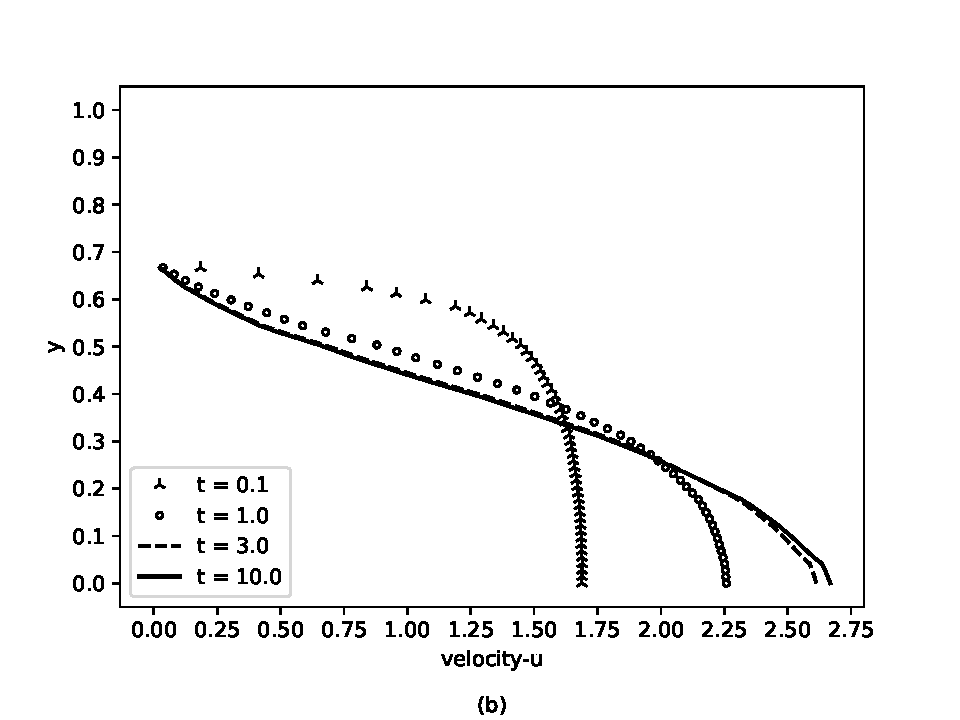
\includegraphics[scale=0.35]{images/vel_RealStrut_evol.pdf}\\
     \end{minipage}
\end{figure}
\vspace{-0.2cm}
\centering \tiny Evolution of velocity profile in centerline ($x=0.5L$):\\
                       (a) Curved Channel and (b) Real Channel
\end{frame}

%%%%%%%%%%%%%%%%%%%%%%%%%%%%%%%%%%%%%%%%%%%%%%%%%%%%%%%%%%%%%%%%%%%%%%%%%%%%%%%%%%%%%%%%%%

\begin{frame}
 \frametitle{\LARGE Results - Concentration Field}
\vspace{-0.7cm}
\begin{figure}
     \begin{minipage}{.50\linewidth}
      \centering
      
\includegraphics[scale=0.075]{images/conc1_CurvedStrut2000.png}\\
      \tiny t = 1.0
     \end{minipage}%
     \begin{minipage}{.50\linewidth}
      \centering
      
\includegraphics[scale=0.075]{images/conc10_CurvedStrut5000.png}\\
      \tiny t = 1.0
     \end{minipage}
     \begin{minipage}{.50\linewidth}
     \medskip
      \centering
      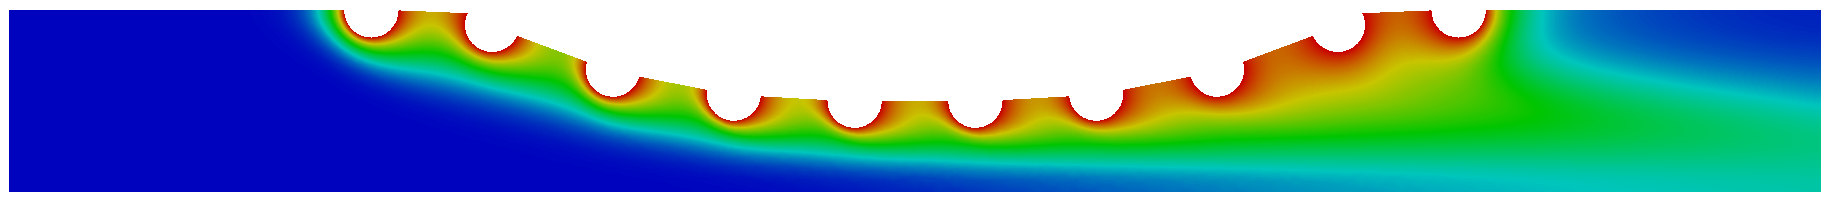
\includegraphics[scale=0.075]{images/conc1_CurvedStrut10000.png}\\
      \tiny t = 5.0
     \end{minipage}%
     \begin{minipage}{.50\linewidth}
     \medskip
      \centering
      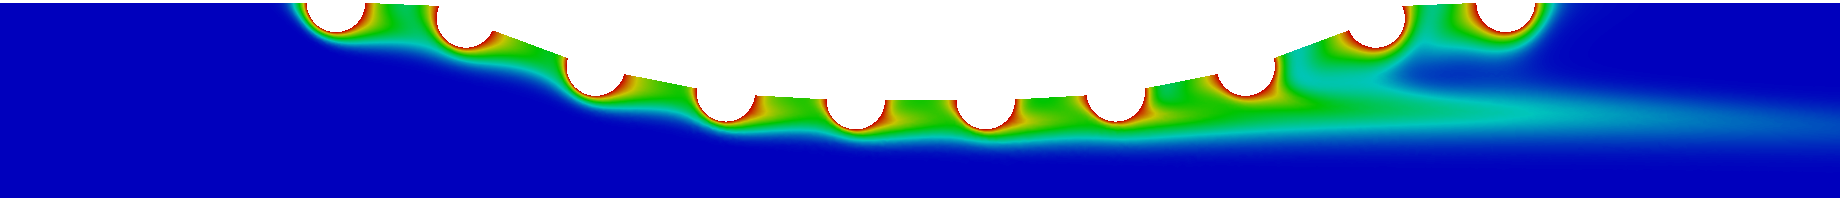
\includegraphics[scale=0.075]{images/conc10_CurvedStrut25000.png}\\
      \tiny t = 5.0
     \end{minipage}
     \begin{minipage}{.50\linewidth}
      \centering
      
\includegraphics[scale=0.075]{images/conc1_CurvedStrut20000.png}\\
      \tiny t = 10.0
     \end{minipage}%
     \begin{minipage}{.50\linewidth}
      \centering
      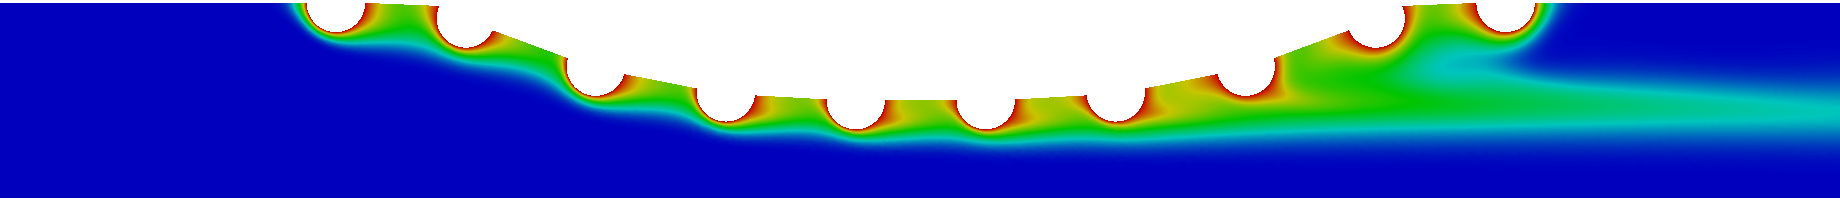
\includegraphics[scale=0.075]{images/conc10_CurvedStrut50000.png}\\
      \tiny t = 10.0
     \end{minipage}
\end{figure}
\vspace{-0.2cm}
\centering \scriptsize Evolution in time and space of concentration field in Curved Channel:\\
                 $Sc=1$ (left column) and $Sc=10$ (right column)
\vspace{0cm}
\begin{figure}
     \begin{minipage}{.50\linewidth}
      \centering
      
\includegraphics[scale=0.075]{images/conc1_RealStrut2000.png}\\
      \tiny t = 1.0
     \end{minipage}%
     \begin{minipage}{.50\linewidth}
      \centering
      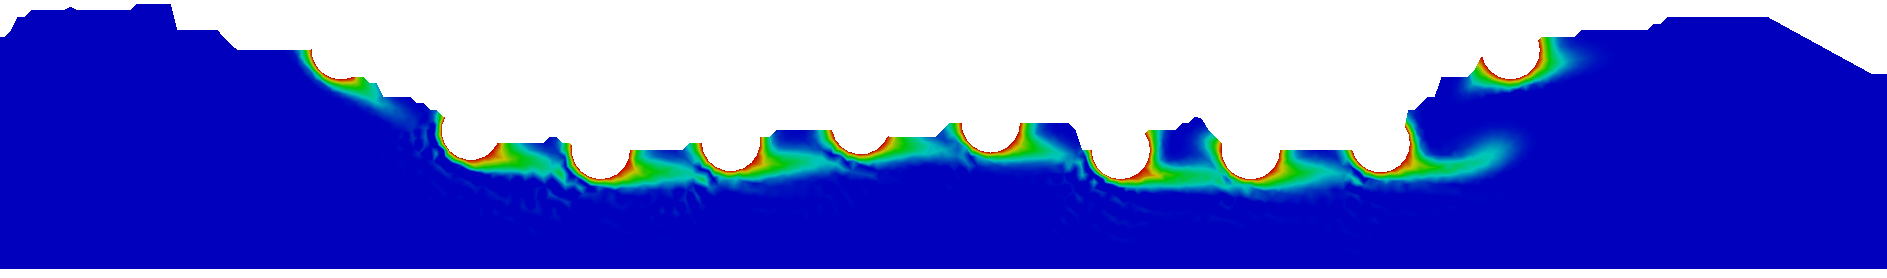
\includegraphics[scale=0.075]{images/conc10_RealStrut5000.png}\\
      \tiny t = 1.0
     \end{minipage}
     \begin{minipage}{.50\linewidth}
     \medskip
      \centering
      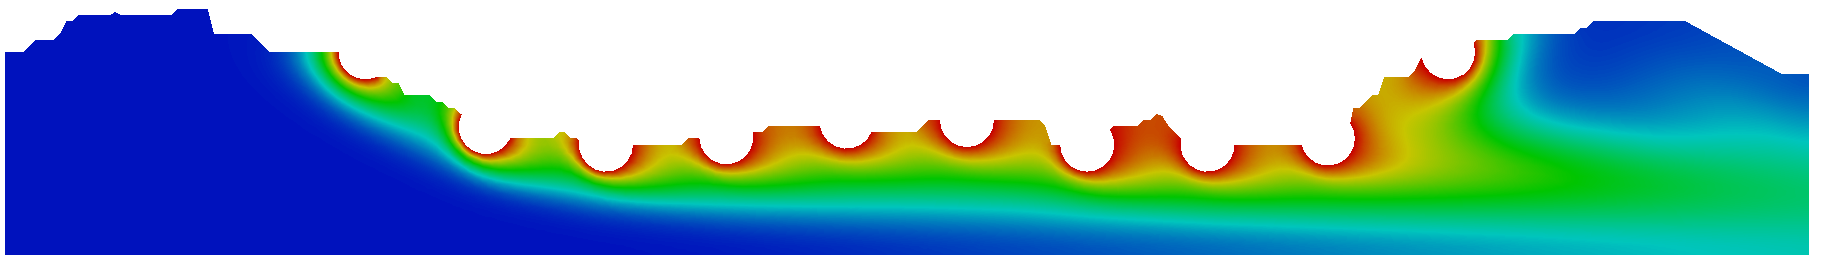
\includegraphics[scale=0.075]{images/conc1_RealStrut10000.png}\\
      \tiny t = 5.0
     \end{minipage}%
     \begin{minipage}{.50\linewidth}
     \medskip
      \centering
      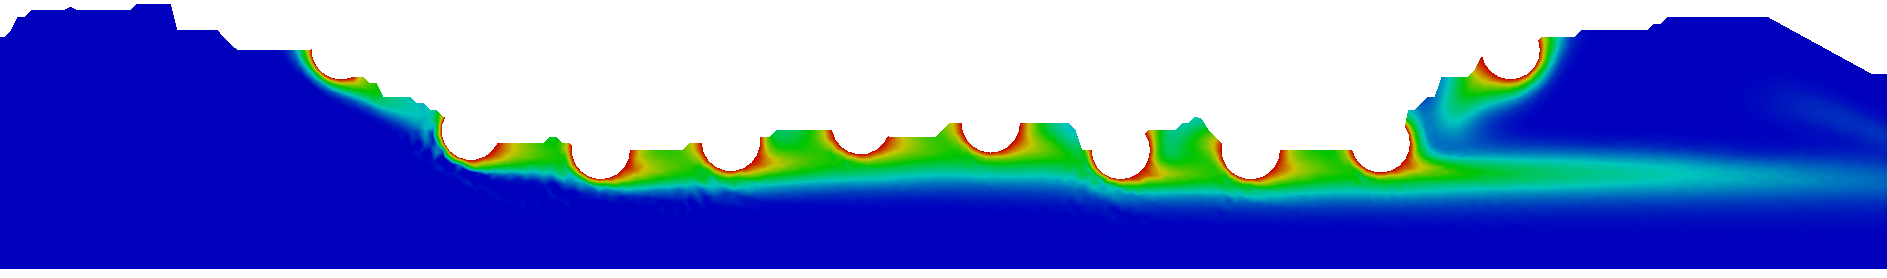
\includegraphics[scale=0.075]{images/conc10_RealStrut25000.png}\\
      \tiny t = 5.0
     \end{minipage}
     \begin{minipage}{.50\linewidth}
      \centering
      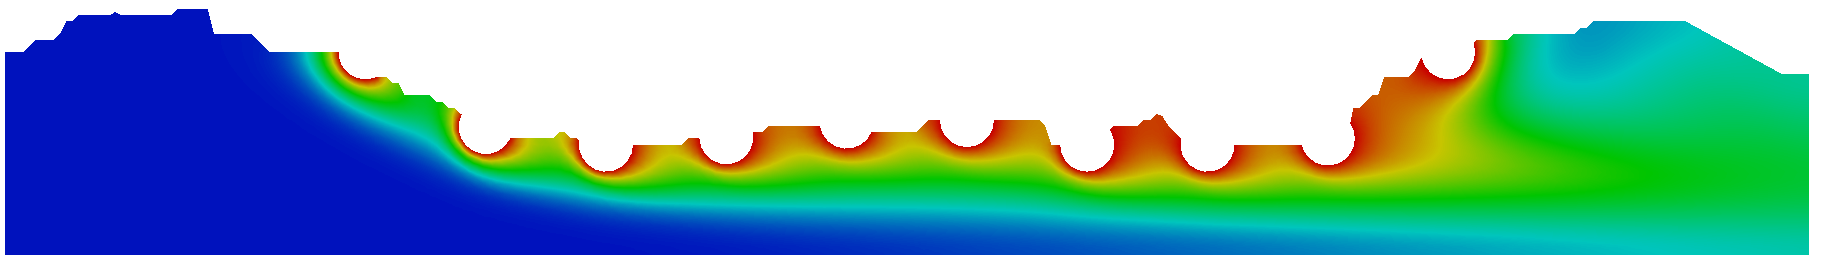
\includegraphics[scale=0.075]{images/conc1_RealStrut20000.png}\\
      \tiny t = 10.0
     \end{minipage}%
     \begin{minipage}{.50\linewidth}
      \centering
      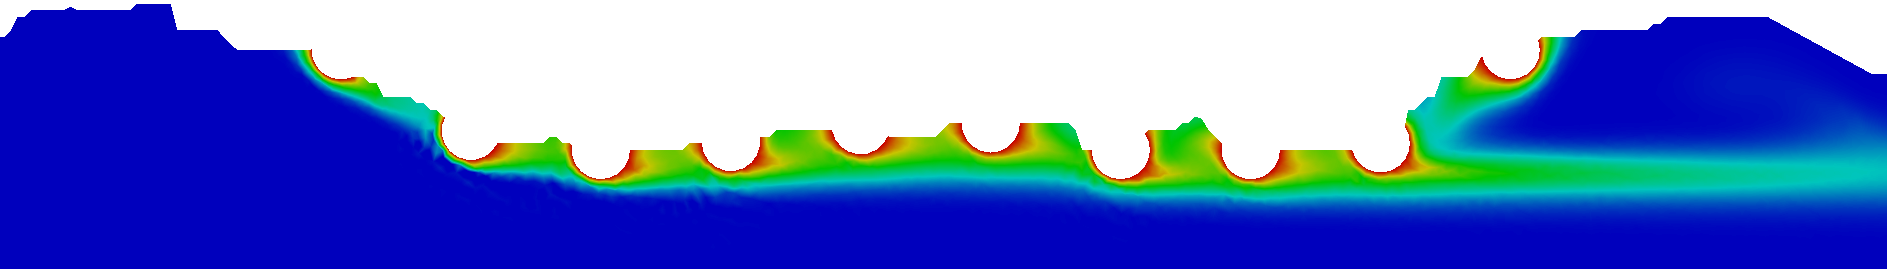
\includegraphics[scale=0.075]{images/conc10_RealStrut50000.png}\\
      \tiny t = 10.0
     \end{minipage}
\end{figure}
\vspace{-0.2cm}
\centering \scriptsize Evolution in time and space of concentration field in Real Channel:\\
                 $Sc=1$ (left column) and $Sc=10$ (right column)
\end{frame}


%%%%%%%%%%%%%%%%%%%%%%%%%%%%%%%%%%%%%%%%%%%%%%%%%%%%%%%%%%%%%%%%%%%%%%%%%%%%%%%%%%%%%%%%%%

\begin{frame}
  \vspace{-1cm}
  \textcolor{gray}{1. Introduction}\\[0.1cm]
  \textcolor{gray}{2. Mathematical Model}\\[0.1cm]
  \textcolor{gray}{3. Validation}\\[0.1cm]
  \textcolor{gray}{4. Results}\\[0.1cm]
  5. Conclusion
\end{frame}


%%%%%%%%%%%%%%%%%%%%%%%%%%%%%%%%%%%%%%%%%%%%%%%%%%%%%%%%%%%%%%%%%%%%%%%%%%%%%%%%%%%%%%%%%%

\begin{frame}
 \frametitle{\LARGE Conclusion}
 \vspace{-1cm}
\begin{enumerate}
 \justifying
 \small
 \item Was observed that the species transport in blood flow is directly influenced
       by drug used in stent production\\

 \vspace{0.3cm}
 
 \item The streamfunction-vorticity formulation showed an useful approach for to calculate
       the velocity and concentration fields since the variables are scalars allowing a
       smooth implementation\\

 \vspace{0.3cm}

 \item Due to generalized construction of the code, the simulator is able to describe
       drug-eluting stent problem in coronary artery as well as flows of Newtonian fluids
       with scalar transport (concentration or temperature)
\end{enumerate}
\end{frame}


%%%%%%%%%%%%%%%%%%%%%%%%%%%%%%%%%%%%%%%%%%%%%%%%%%%%%%%%%%%%%%%%%%%%%%%%%%%%%%%%%%%%%%%%%%

\begin{frame}
 \centering
 \vspace{-1cm}
 \Huge Thank you!\\
 \vspace{0.5cm}
 \small marquesleandro67@gmail.com\\
 \small jose.pontes@uerj.br\\
 \small gustavo.rabello@mecanica.coppe.ufrj.br\\
 \vspace{1.0cm}
 \small The authors thank the FAPERJ (Research Support Foundation of the State of Rio de Janeiro)
        for its financial support

 \vspace{-0.2cm}
 \begin{figure}
  \centering
  
\includegraphics[scale=0.4]{images/faperj.jpg}\\
 \end{figure}
\end{frame}




\end{document}
%%%%%%%%%%%%%%%%%%%%%%%%%%%%%%%%%%%%%%%%%%%%%%%%%%%%%%%%%%%%%%%%%%%%%%%%%%%%%%%%%%%%%%%%%%
